\documentclass[xetex,mathsans,sans,aspectratio=169]{beamer}
\usepackage{listings}
\usetheme{Boadilla}
\usecolortheme{orchid}
\usepackage{fontspec}
\setsansfont{Basis Grotesque}
\setbeamertemplate{navigation symbols}{}
\usepackage{amsmath}
\usepackage{multicol}

% The title slide information about the presenter(s) eg. name(s), role(s)
\newcommand{\presenter}{<presenter name(s), role(s)>}

% The text for the presenter footer eg. first name(s)
\newcommand{\presenterfooter}{<presenter fname(s)>}

% The footer title of the presentation (optional - default is 'NuCypher')
\newcommand{\titlefooter}{NuCypher}

% The email name prefix for the presenter i.e. <email_prefix>@nucypher.com
\newcommand{\emailname}{<email\_prefix>}

% The name of the event
\newcommand{\event}{<event name>}

% The date of the event with format: dd MMM yyyy
\newcommand{\eventdate}{<dd MMM yyyy>}


% Example usage:
%
%     \newcommand{\presenter}{MacLane Wilkison, CEO \& Co-Founder}
%     \newcommand{\presenterfooter}{MacLane}
%     \newcommand{\titlefooter}{NuCypher}
%     \newcommand{\emailname}{maclane}
%     \newcommand{\event}{Eth SF}
%     \newcommand{\eventdate}{05 Oct 2018}
%


\title[\titlefooter]{}
\author[\presenterfooter]{}
\date[\eventdate]{}

\begin{document}
    {
        \usebackgroundtemplate{\includegraphics[width=\paperwidth]{pdf/cryptocamp_title_page.pdf}}
        \begin{frame}
            \titlepage
        \end{frame}
    }

    \begin{frame}
      \frametitle{NuCypher Overview}
        \begin{itemize}
            \item Use cryptography to build the tools \& infrastructure to preserve data privacy
            \item Privacy-preserving solutions for distributed applications
              \begin{itemize}
                  \item Proxy Re-encryption (PRE)
                  \begin{itemize}
                    \item Secure data-sharing and access control of encrypted data
                  \end{itemize}
                  \item Fully Homomorphic Encryption (FHE)
                  \begin{itemize}
                    \item Perform arbitrary operations on encrypted data
                  \end{itemize}
              \end{itemize}
            \item Blockchain \& Private Deployments
        \end{itemize}
    \end{frame}

    \begin{frame}
      \frametitle{Problem}
      \framesubtitle{Data Breaches}
        \begin{figure}
            \centering
            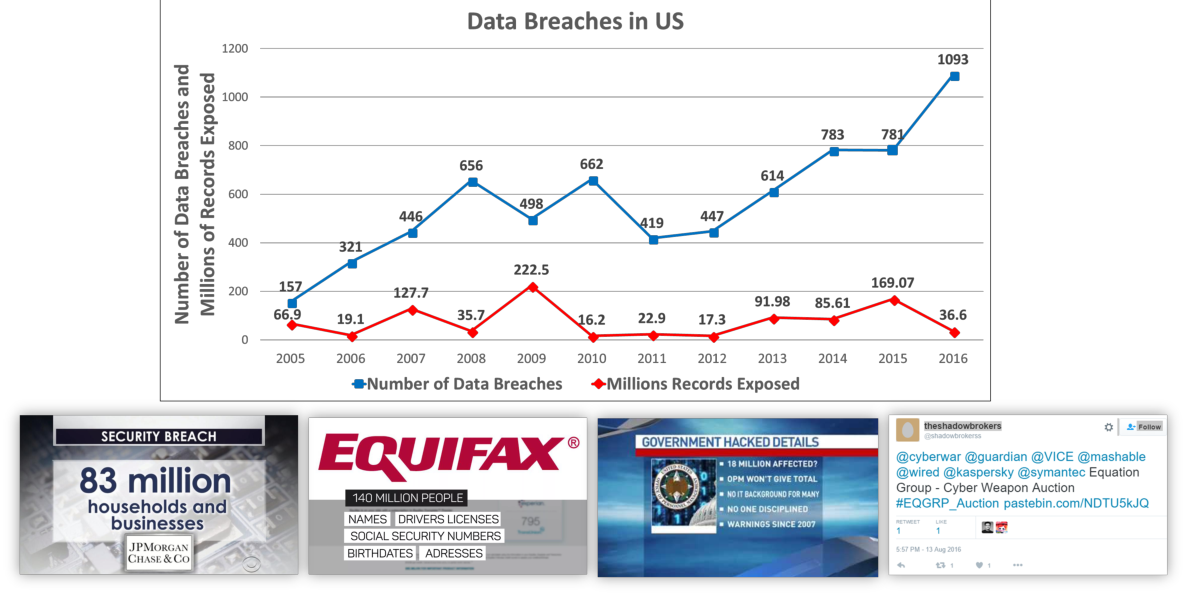
\includegraphics[height=6cm]{pdf/data-breaches.pdf}
        \end{figure}

        {\tiny Source: \url{https://www.statista.com/statistics/273550/data-breaches-recorded-in-the-united-states-by-number-of-breaches-and-records-exposed/} \par}
    \end{frame}

    \begin{frame}
        \frametitle{Public Key Encryption (PKE)}
        \begin{figure}
            \centering
            \includegraphics<1>[width=11cm]{pdf/pke-multi.pdf}
            \includegraphics<2>[width=11cm]{pdf/pke-multi-hack.pdf}
        \end{figure}

        Limitations
        \begin{itemize}
            \item<2> Decryption required before sharing
            \item<2> Not scalable
            \item<2> Complex access revocation
        \end{itemize}
    \end{frame}

    \begin{frame}
        \frametitle{What is proxy re-encryption (PRE)}
        \begin{figure}
            \centering
            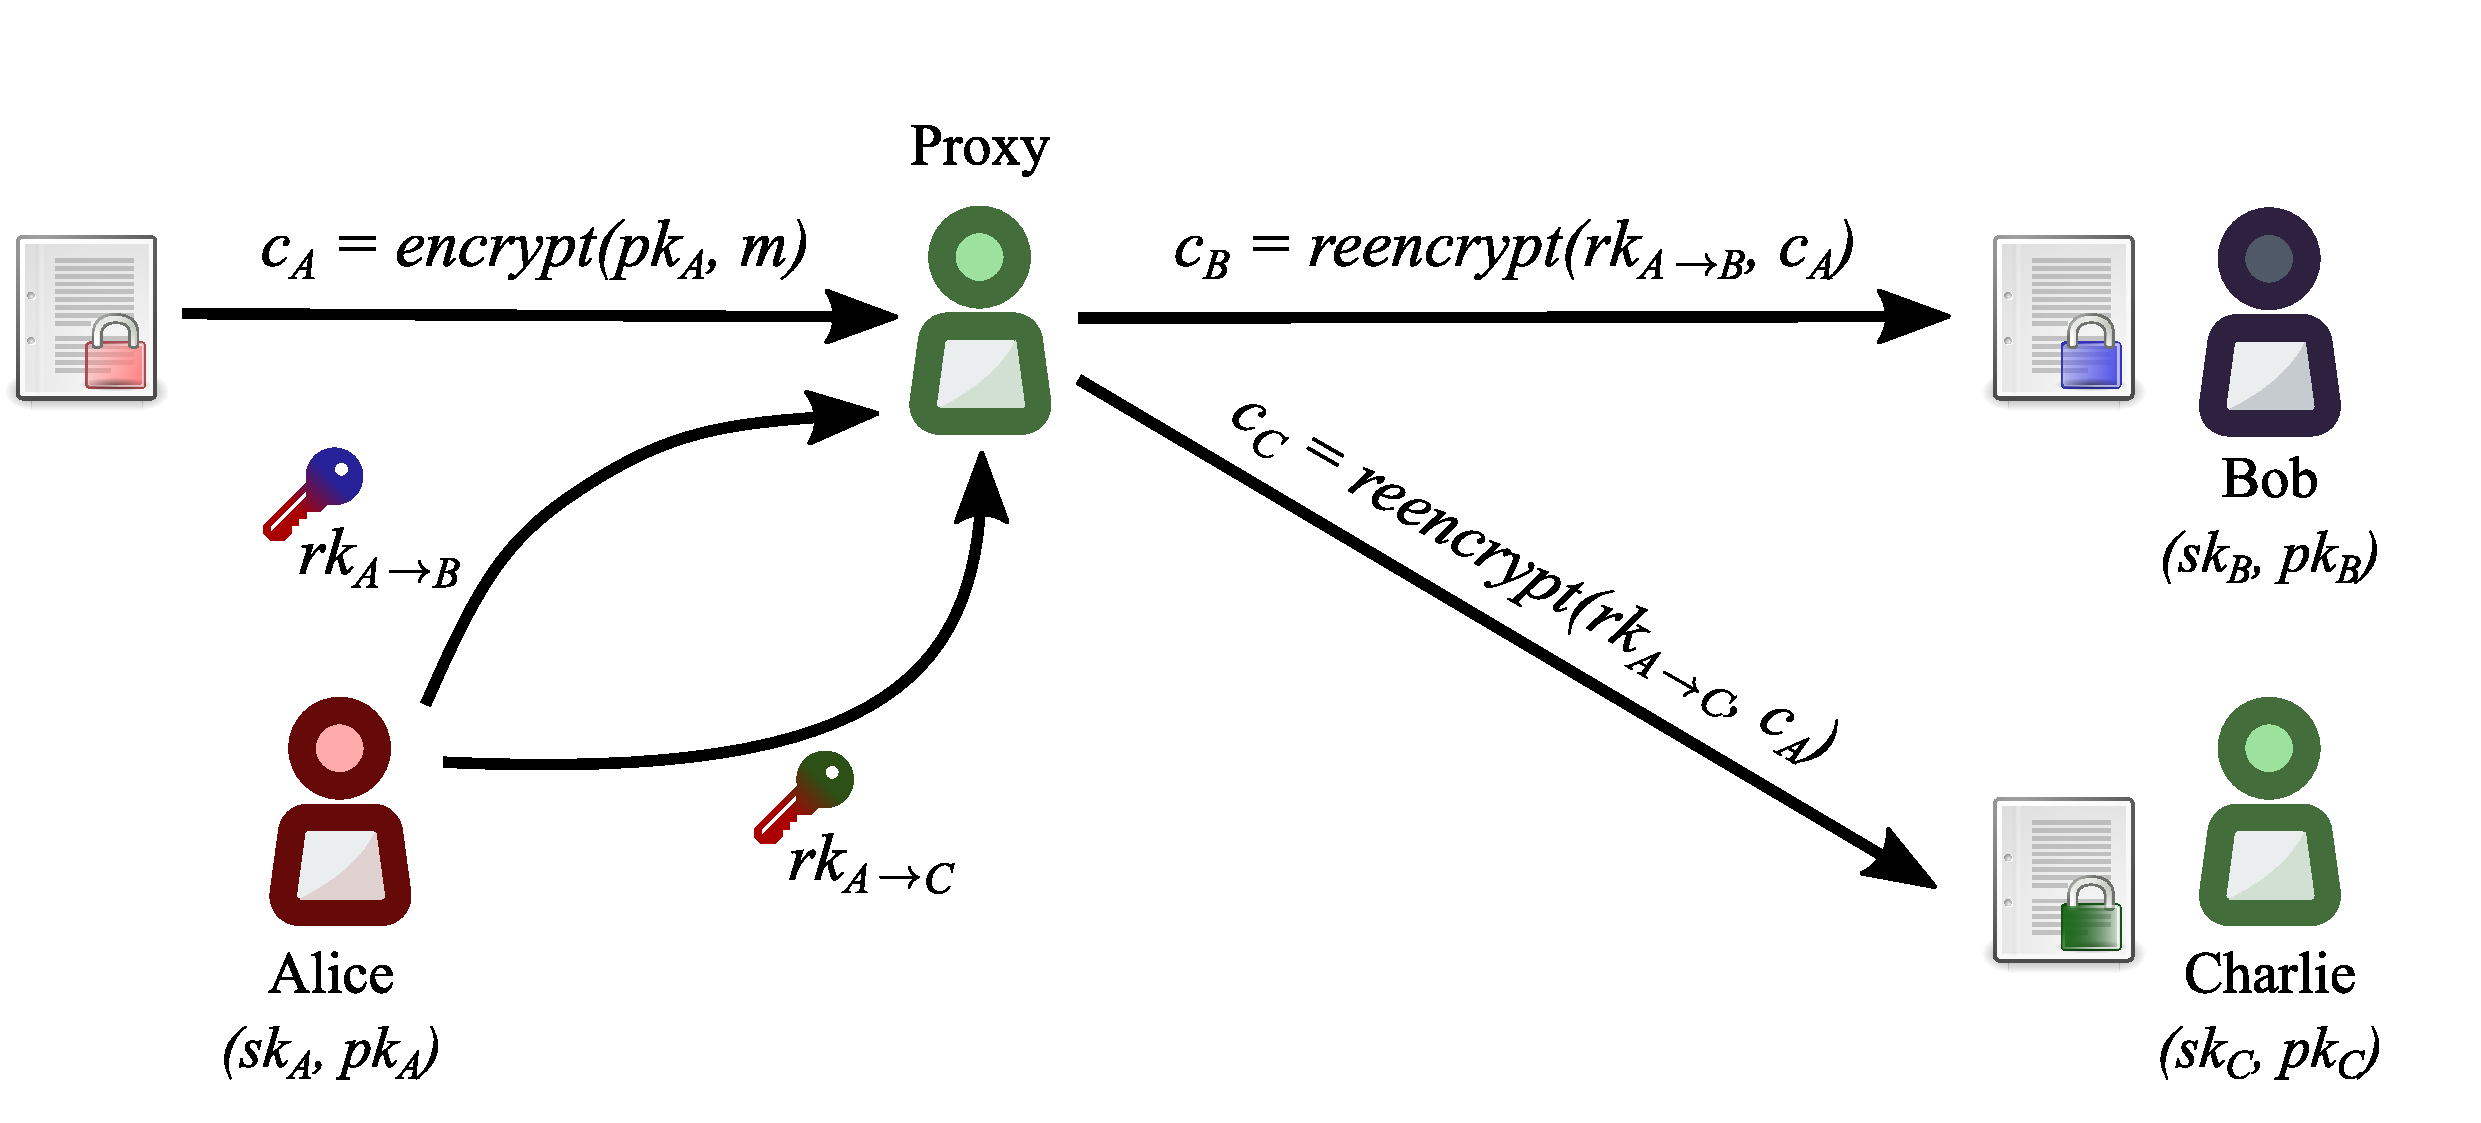
\includegraphics[width=13cm]{pdf/pre-multi.pdf}
        \end{figure}
    \end{frame}

    \begin{frame}
        \frametitle{Solution}
        \framesubtitle{Proxy Re-encryption + Key Management}
        \begin{figure}
            \centering
            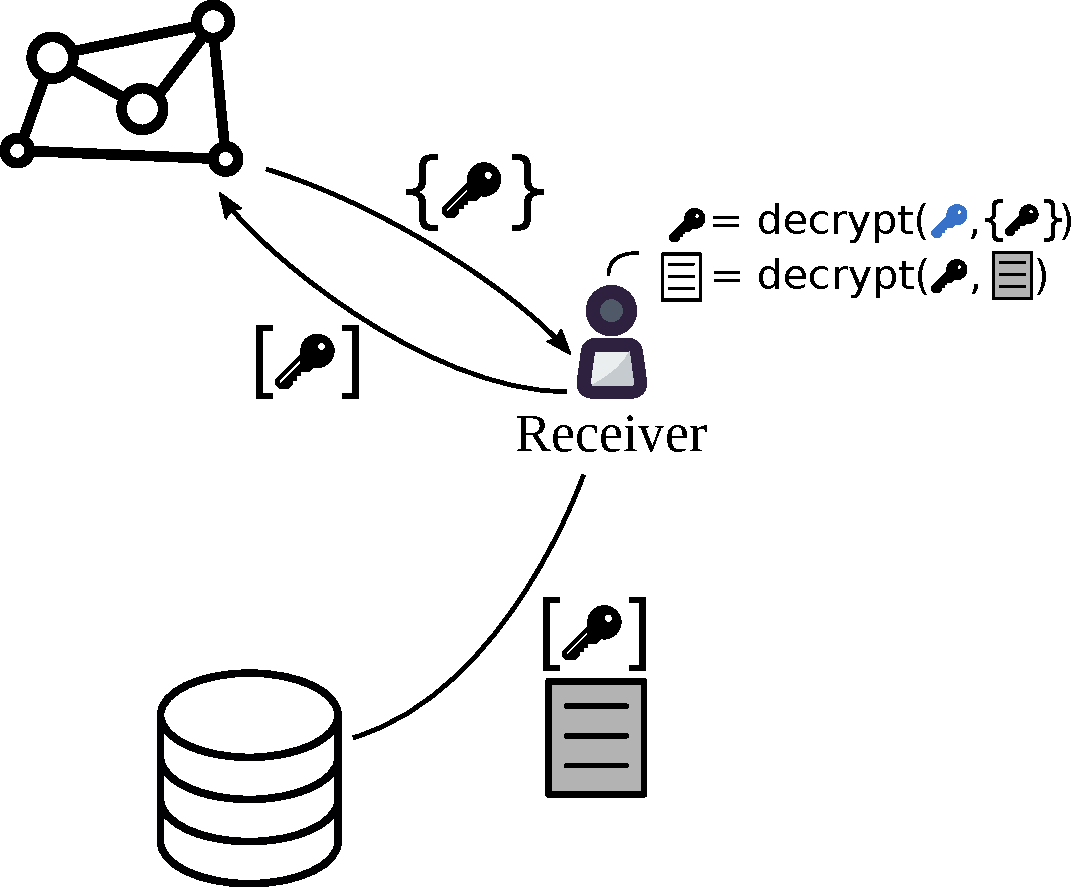
\includegraphics[height=4.5cm]{pdf/pre-kms.pdf}
        \end{figure}

        Advantages
        \begin{itemize}
            \item Data not decrypted to facilitate sharing
            \item Scalable and performant
            \item Access revocation through re-encryption key deletion
            \item Secure use of data storage providers
        \end{itemize}
    \end{frame}

    \begin{frame}
        \frametitle{Centralized KMS using PRE}
        \framesubtitle{Encryption}
        \begin{figure}
            \centering
            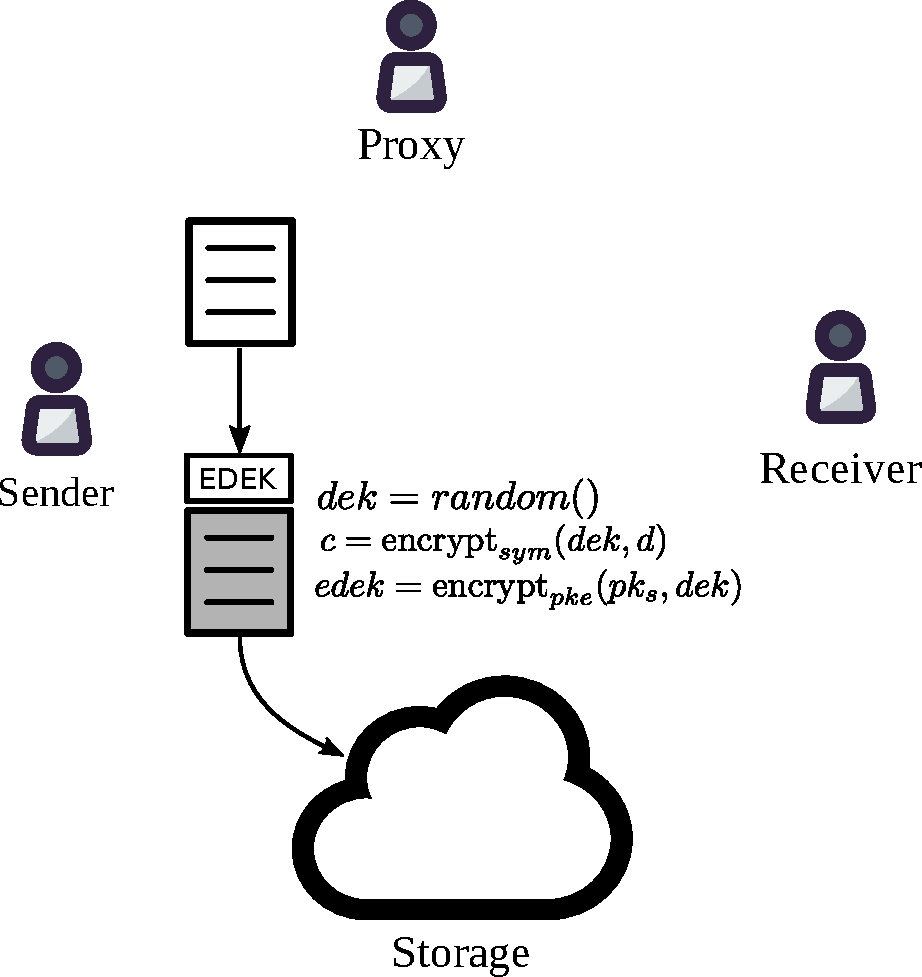
\includegraphics[height=7cm]{pdf/encrypt.pdf}
        \end{figure}
    \end{frame}

    \begin{frame}
        \frametitle{Centralized KMS using PRE}
        \framesubtitle{Access delegation}
        \begin{figure}
            \centering
            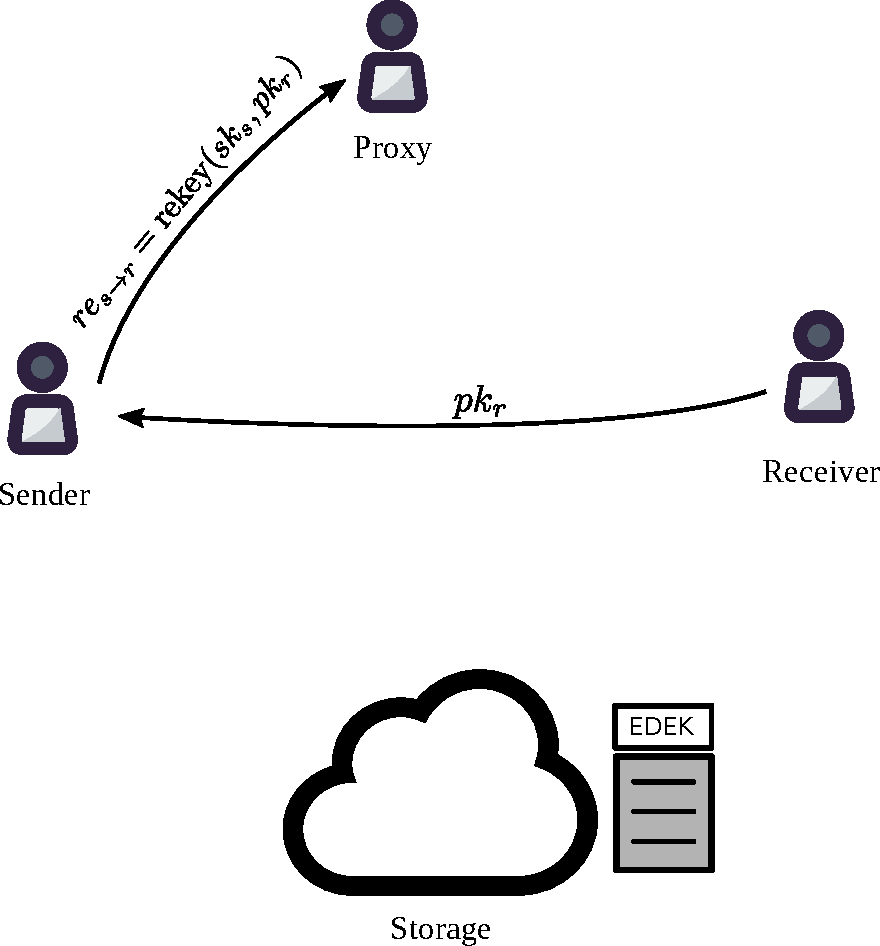
\includegraphics[height=7cm]{pdf/delegate.pdf}
        \end{figure}
    \end{frame}

    \begin{frame}
        \frametitle{Centralized KMS using PRE}
        \framesubtitle{Decryption}
        \begin{figure}
            \centering
            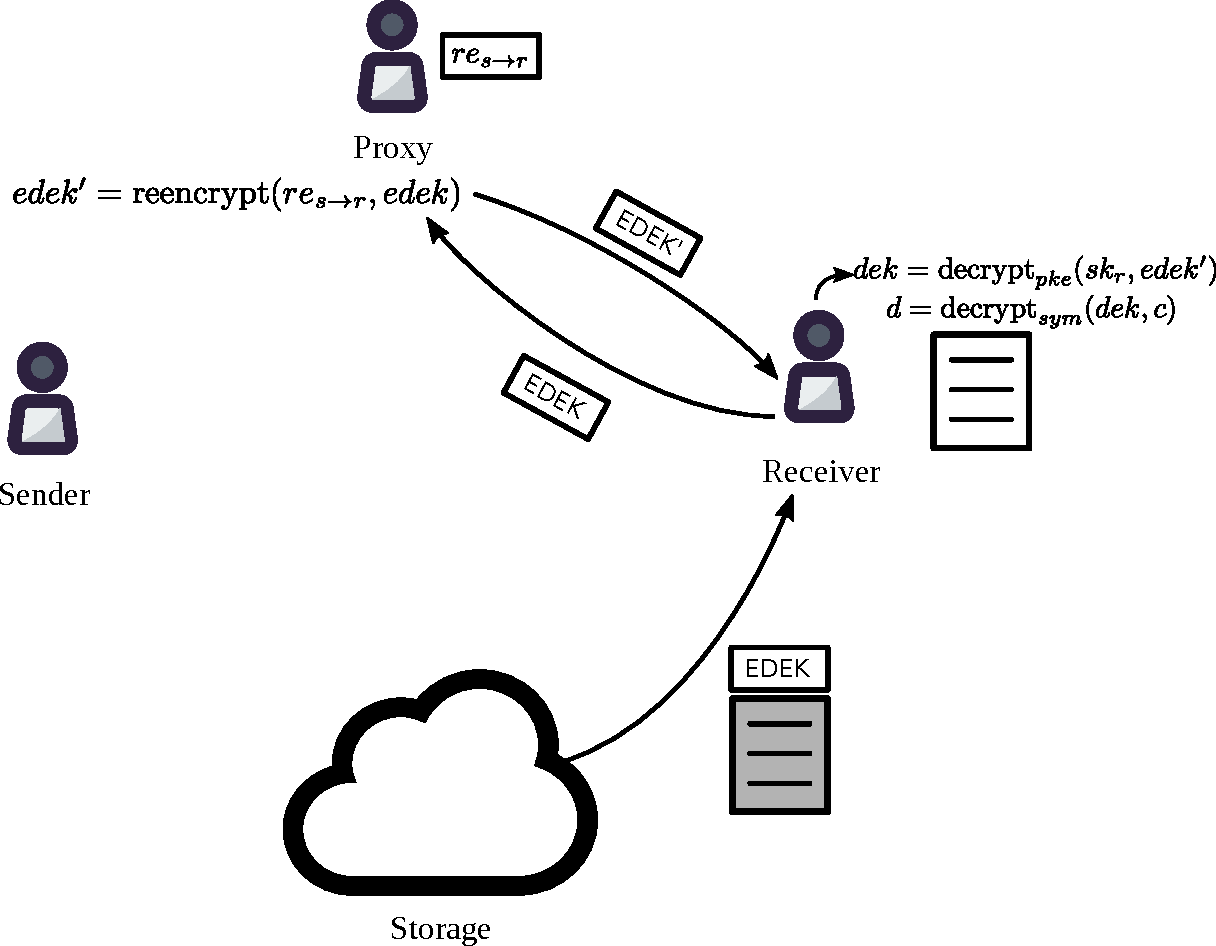
\includegraphics[height=7cm]{pdf/decrypt.pdf}
        \end{figure}
    \end{frame}

    \begin{frame}
        \frametitle{Decentralized KMS using PRE}
        \framesubtitle{Using threshold split-key re-encryption (Umbral)}
        \begin{figure}
            \centering
            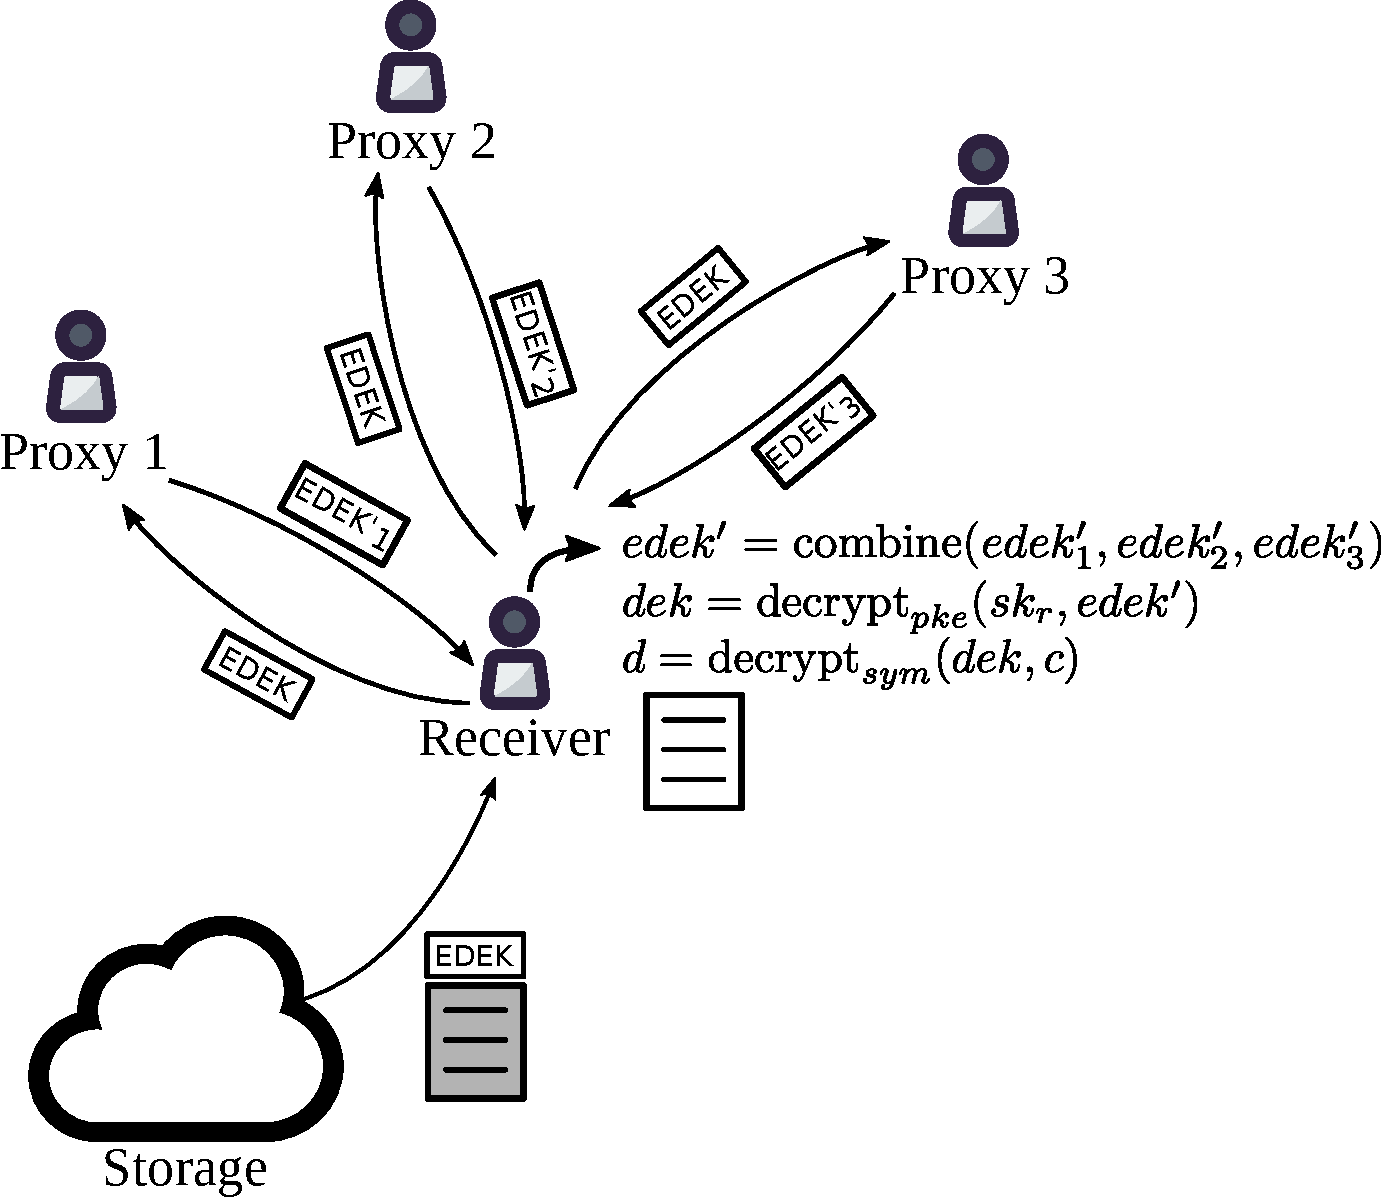
\includegraphics[height=6cm]{pdf/decrypt-umbral.pdf}
        \end{figure}
    \end{frame}

    \begin{frame}
      \frametitle{Umbral Flow Diagram}
      \begin{figure}
        \centering
        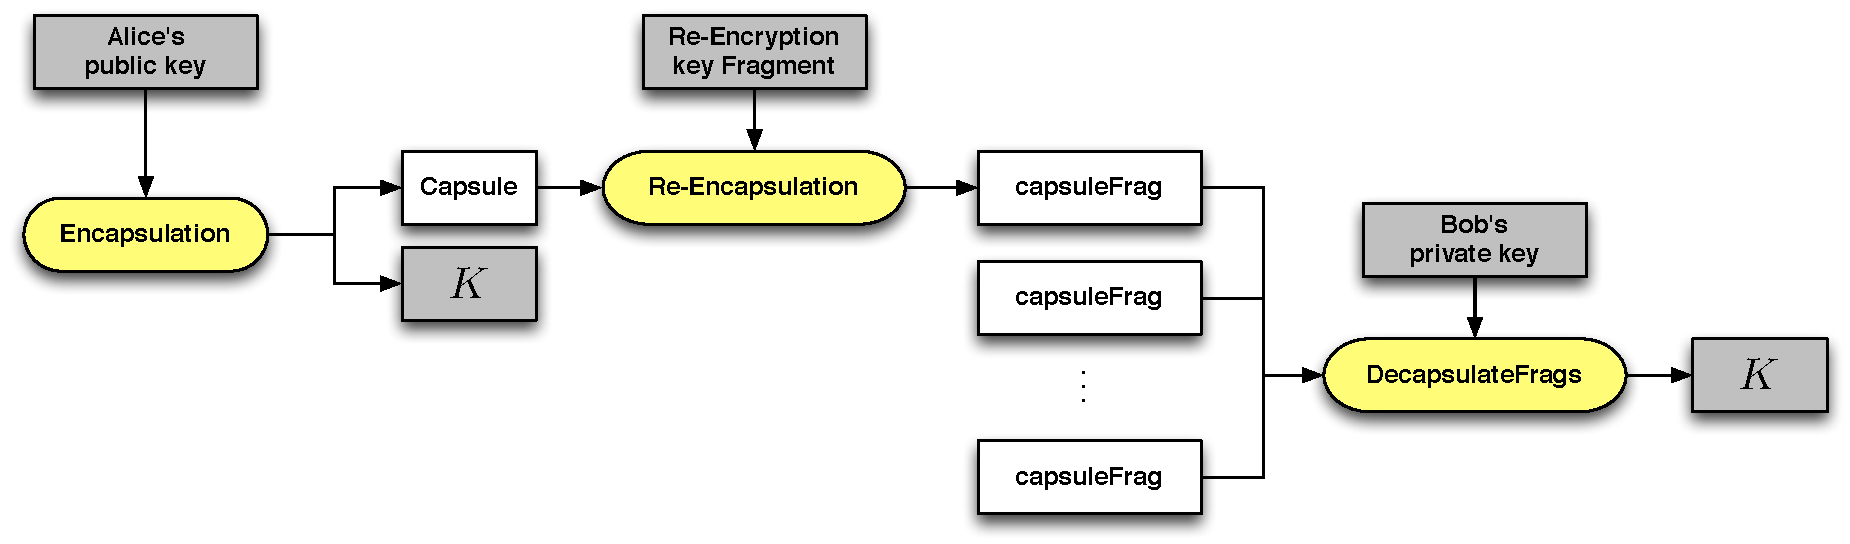
\includegraphics[width=11cm]{pdf/umbral-kem-flow.pdf}
      \end{figure}
      \begin{itemize}
           \item Documentation: \url{https://github.com/nucypher/umbral-doc}
           \item Reference implementation: \url{https://github.com/nucypher/pyUmbral}
      \end{itemize}
    \end{frame}

    \begin{frame}
        \frametitle{Decentralized KMS: Token}
        \framesubtitle{Purpose}
        \begin{itemize}
            \item Splitting trust across re-encryption nodes 
            \begin{itemize}
              \item More tokens = more trust, more work, and more compensation
            \end{itemize}
            \item Proof of Stake for minting new coins according to the mining schedule
            \item Security deposit at stake against malicious behavior of nodes
        \end{itemize}
    \end{frame}

   \begin{frame}
        \frametitle{Data Sharing Policies}
        \begin{itemize}
            \item Time-based
            \item Conditional on payment 
            \begin{itemize}
              \item ``Grant access once paid, continue granting while paying''
            \end{itemize}
            \item Smart contract (public) method
        \end{itemize}
        Decentralized re-encryption nodes (Ursulas) relied on to apply conditions without having the ability to decrypt data
    \end{frame}

    \begin{frame}
        \frametitle{Blockchain \& Smart Contract Agnostic}
        \begin{figure}
            \centering
            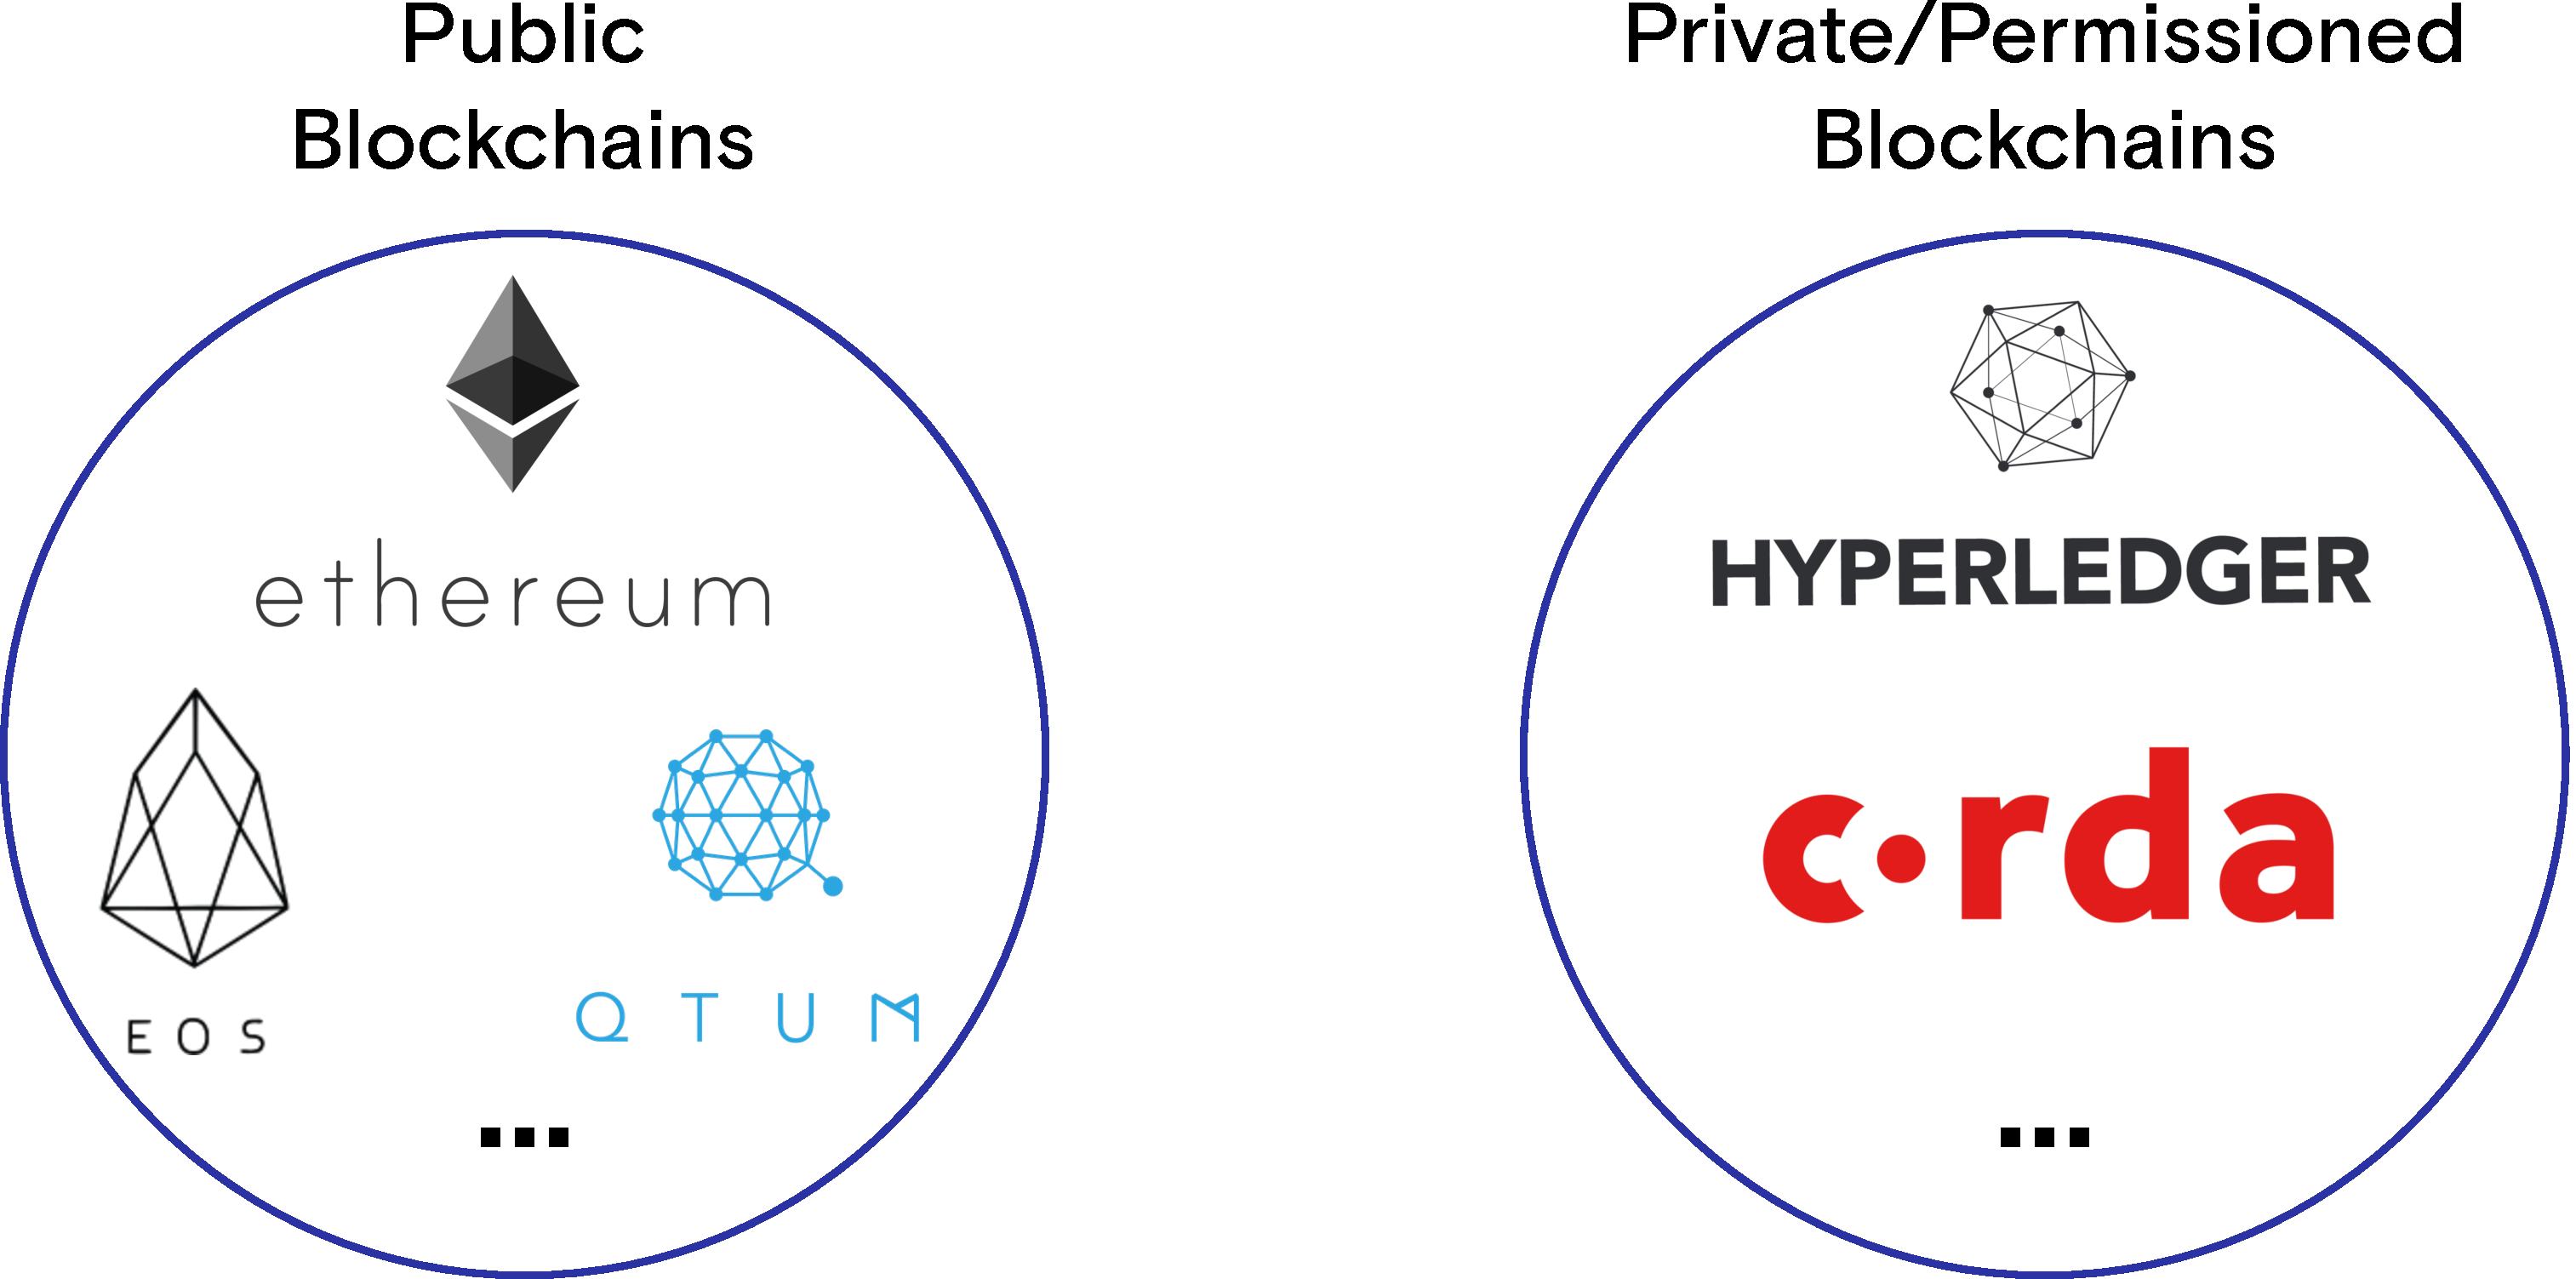
\includegraphics[height=6cm]{pdf/blockchains.pdf}
        \end{figure}
    \end{frame}

    \begin{frame}
        \frametitle{Use Cases}
        \framesubtitle{Scalable, Secure IOT Updates}
        \begin{figure}
            \centering
            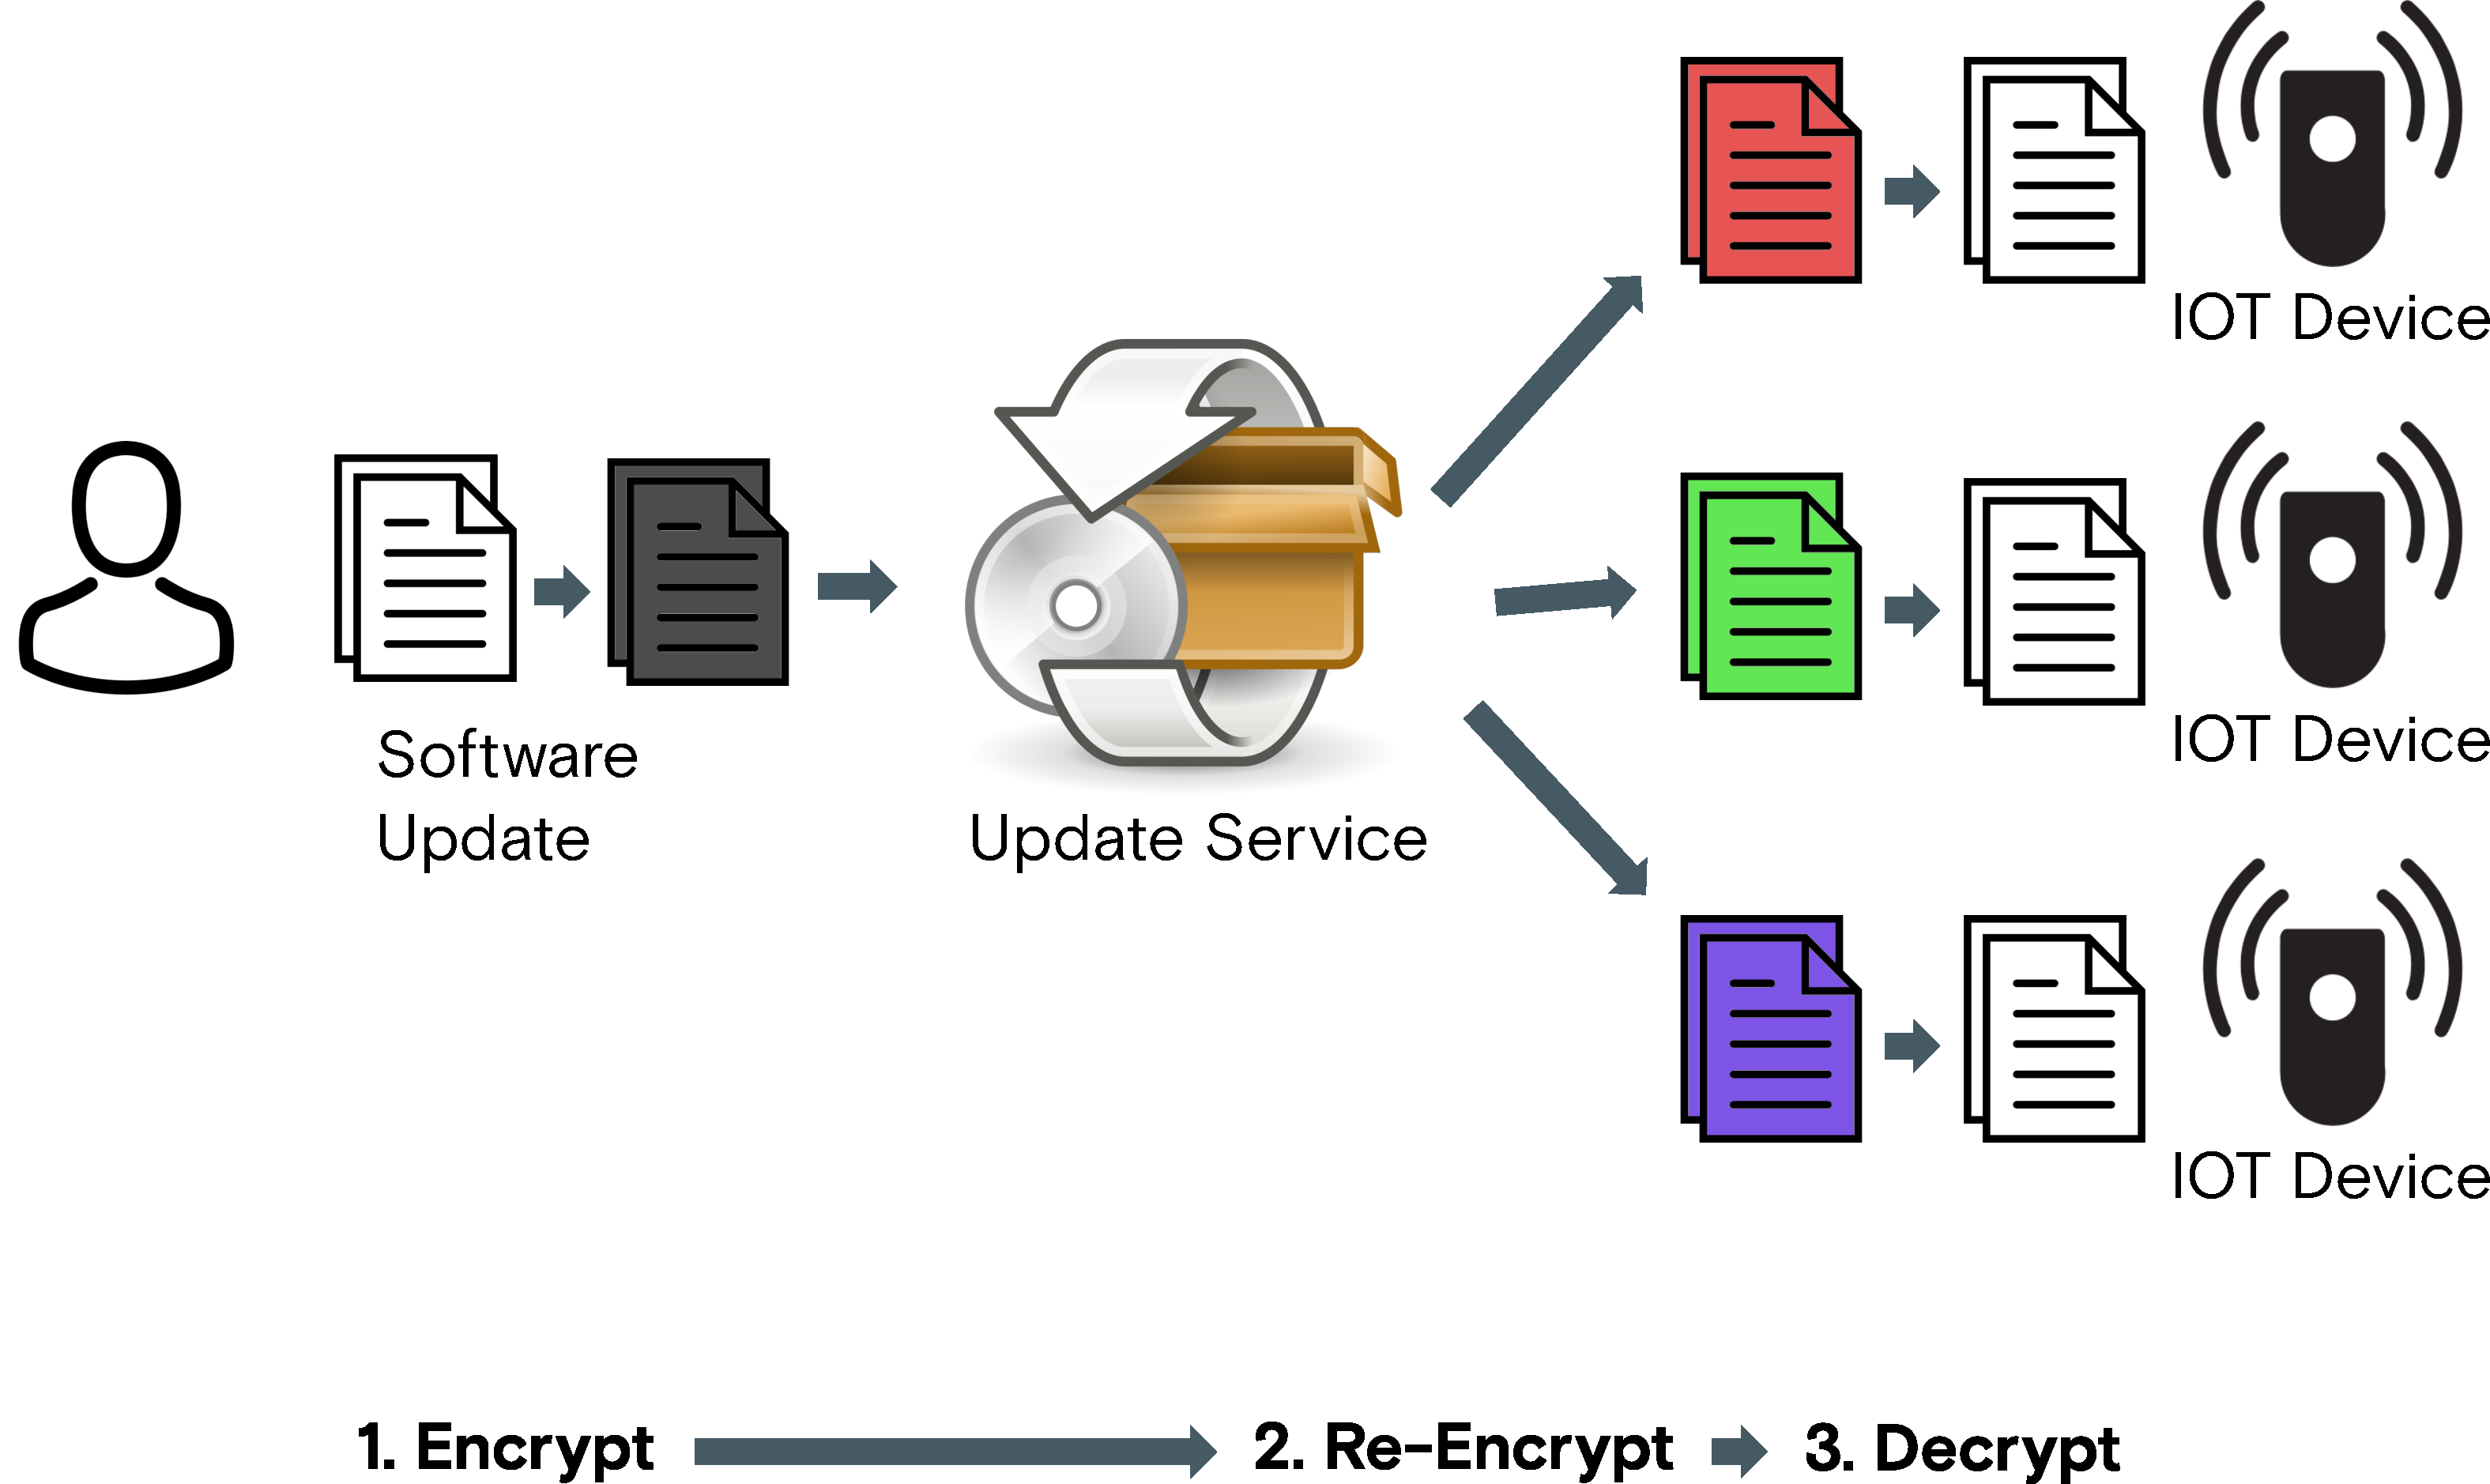
\includegraphics[height=7cm]{pdf/iot-updates-alternative.pdf}
        \end{figure}
    \end{frame}

    \begin{frame}
        \frametitle{Use Cases}
        \framesubtitle{Encrypted file sharing}
        \begin{figure}
            \centering
            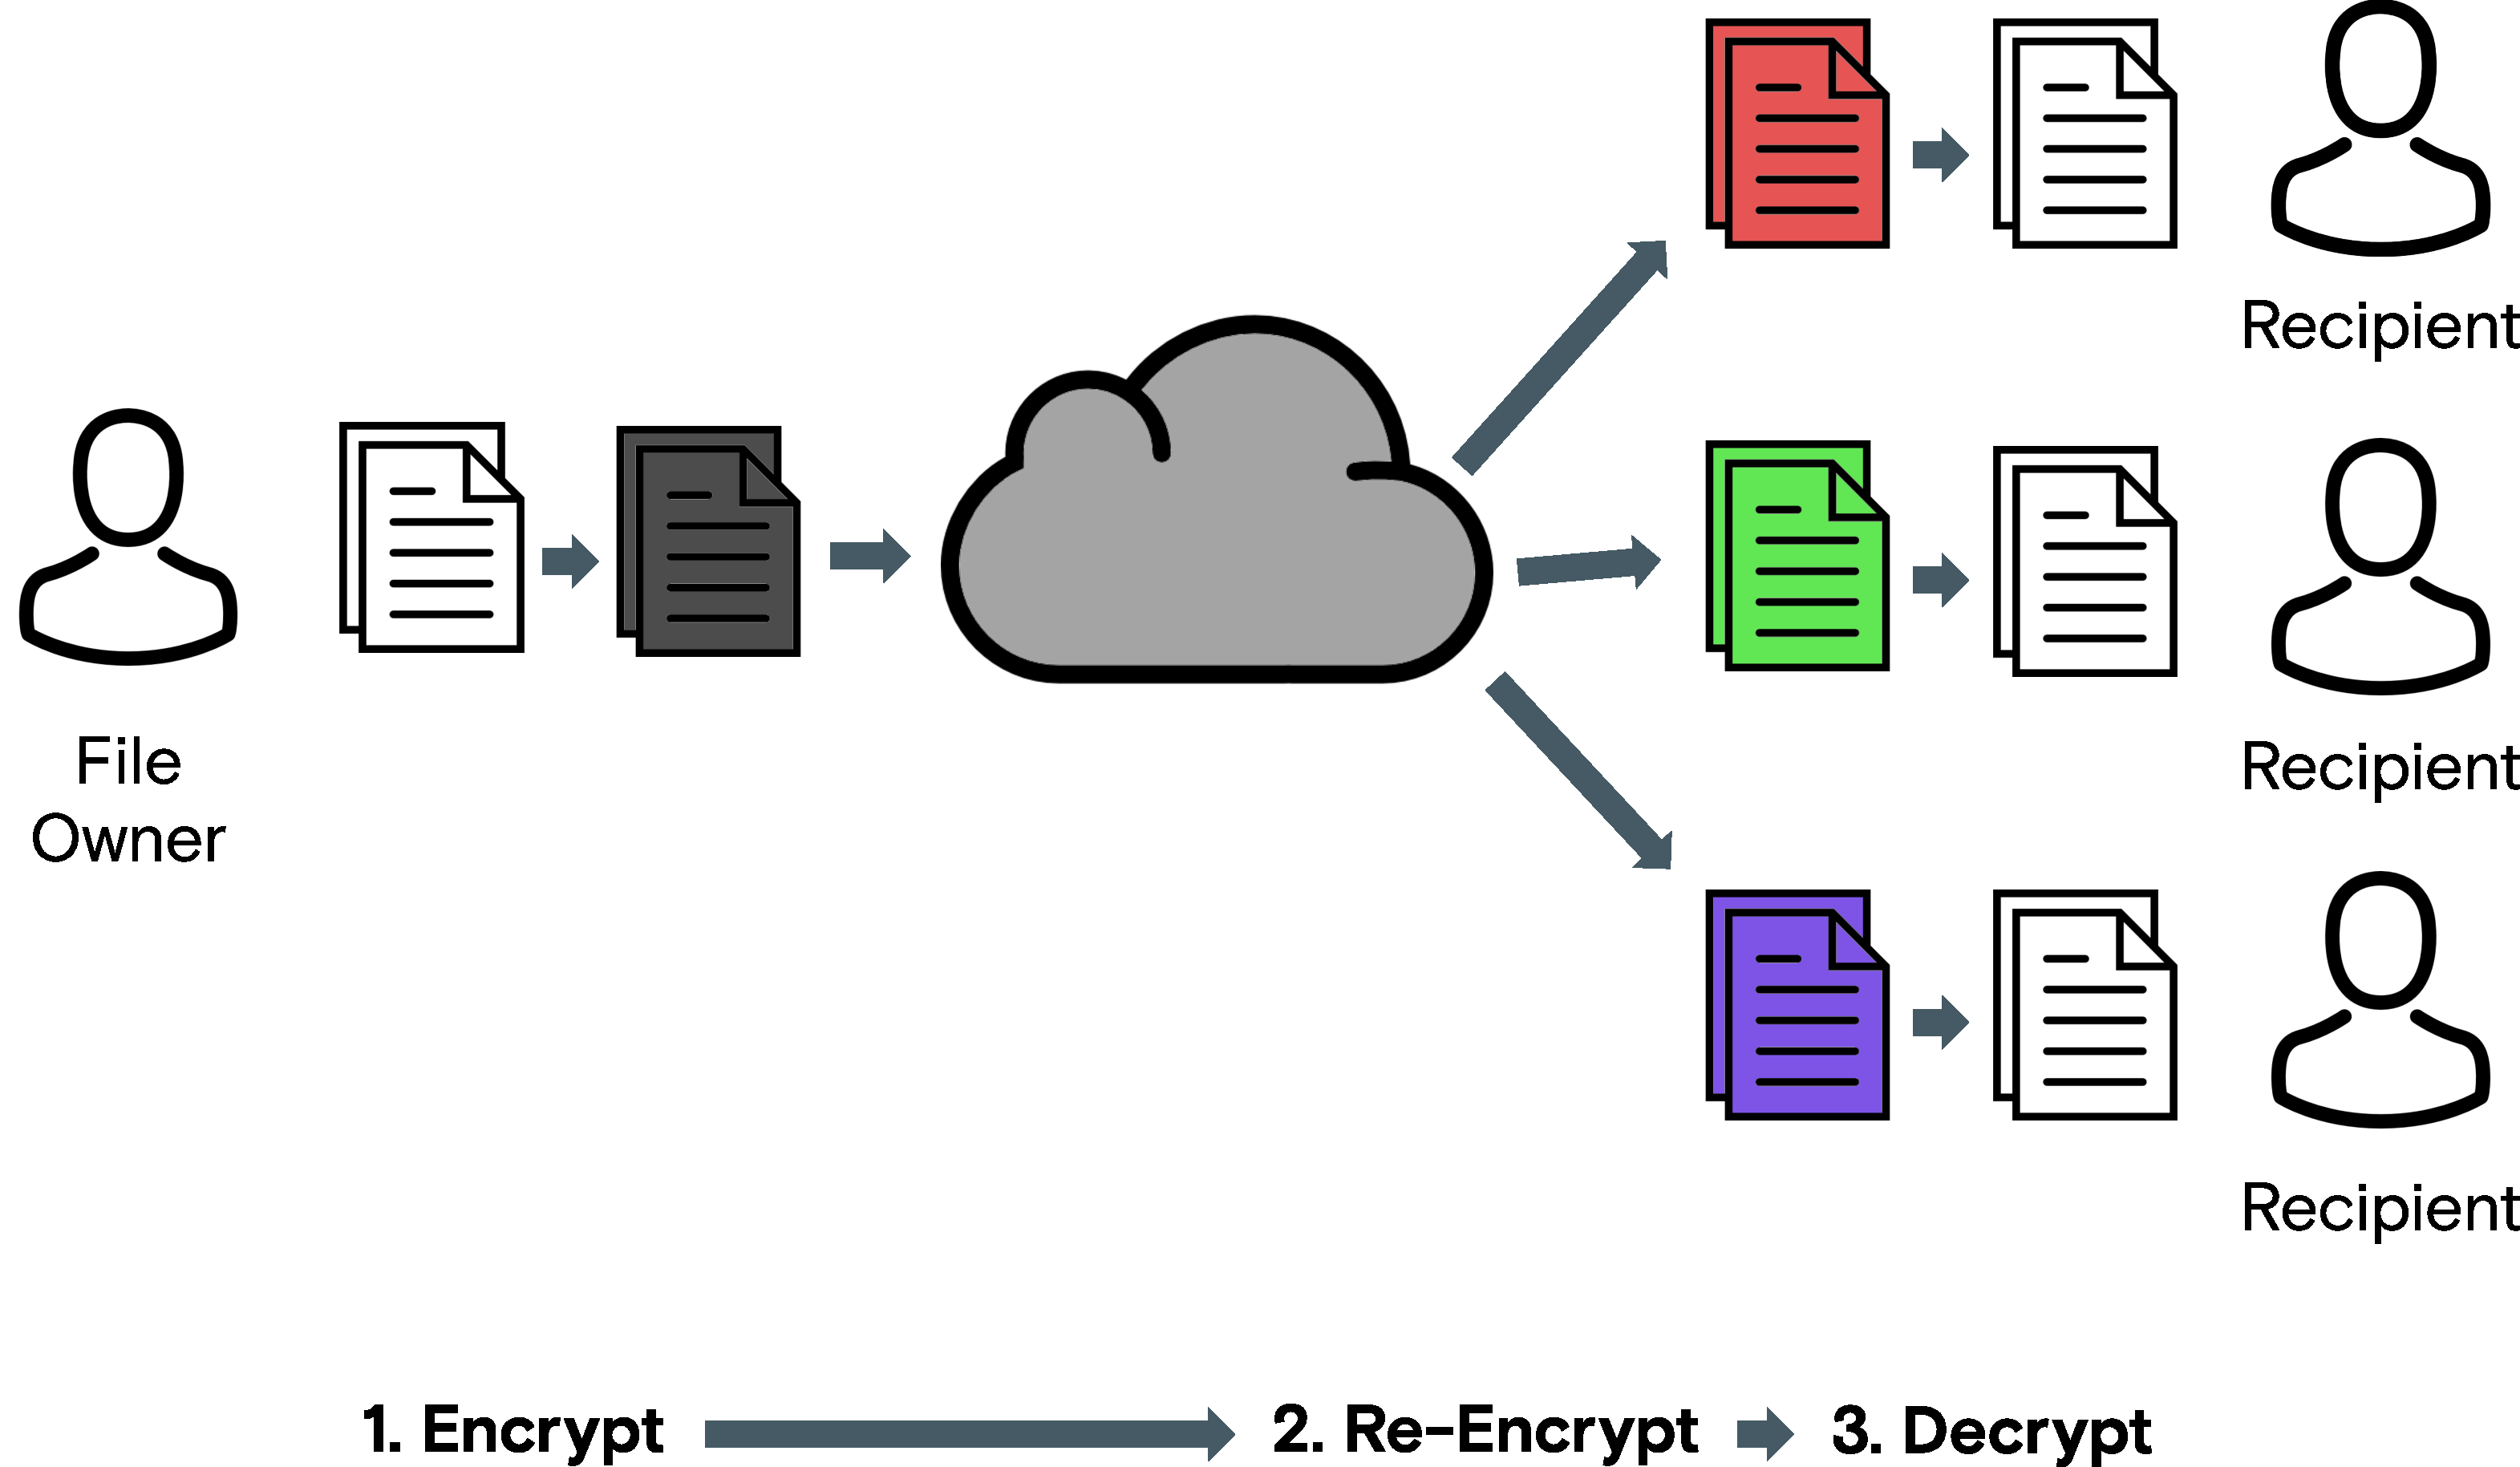
\includegraphics[height=7cm]{pdf/file-sharing-alternative.pdf}
        \end{figure}
    \end{frame}

    \begin{frame}
        \frametitle{Use Cases}
        \framesubtitle{Encrypted multi-user chats}
        \begin{figure}
            \centering
            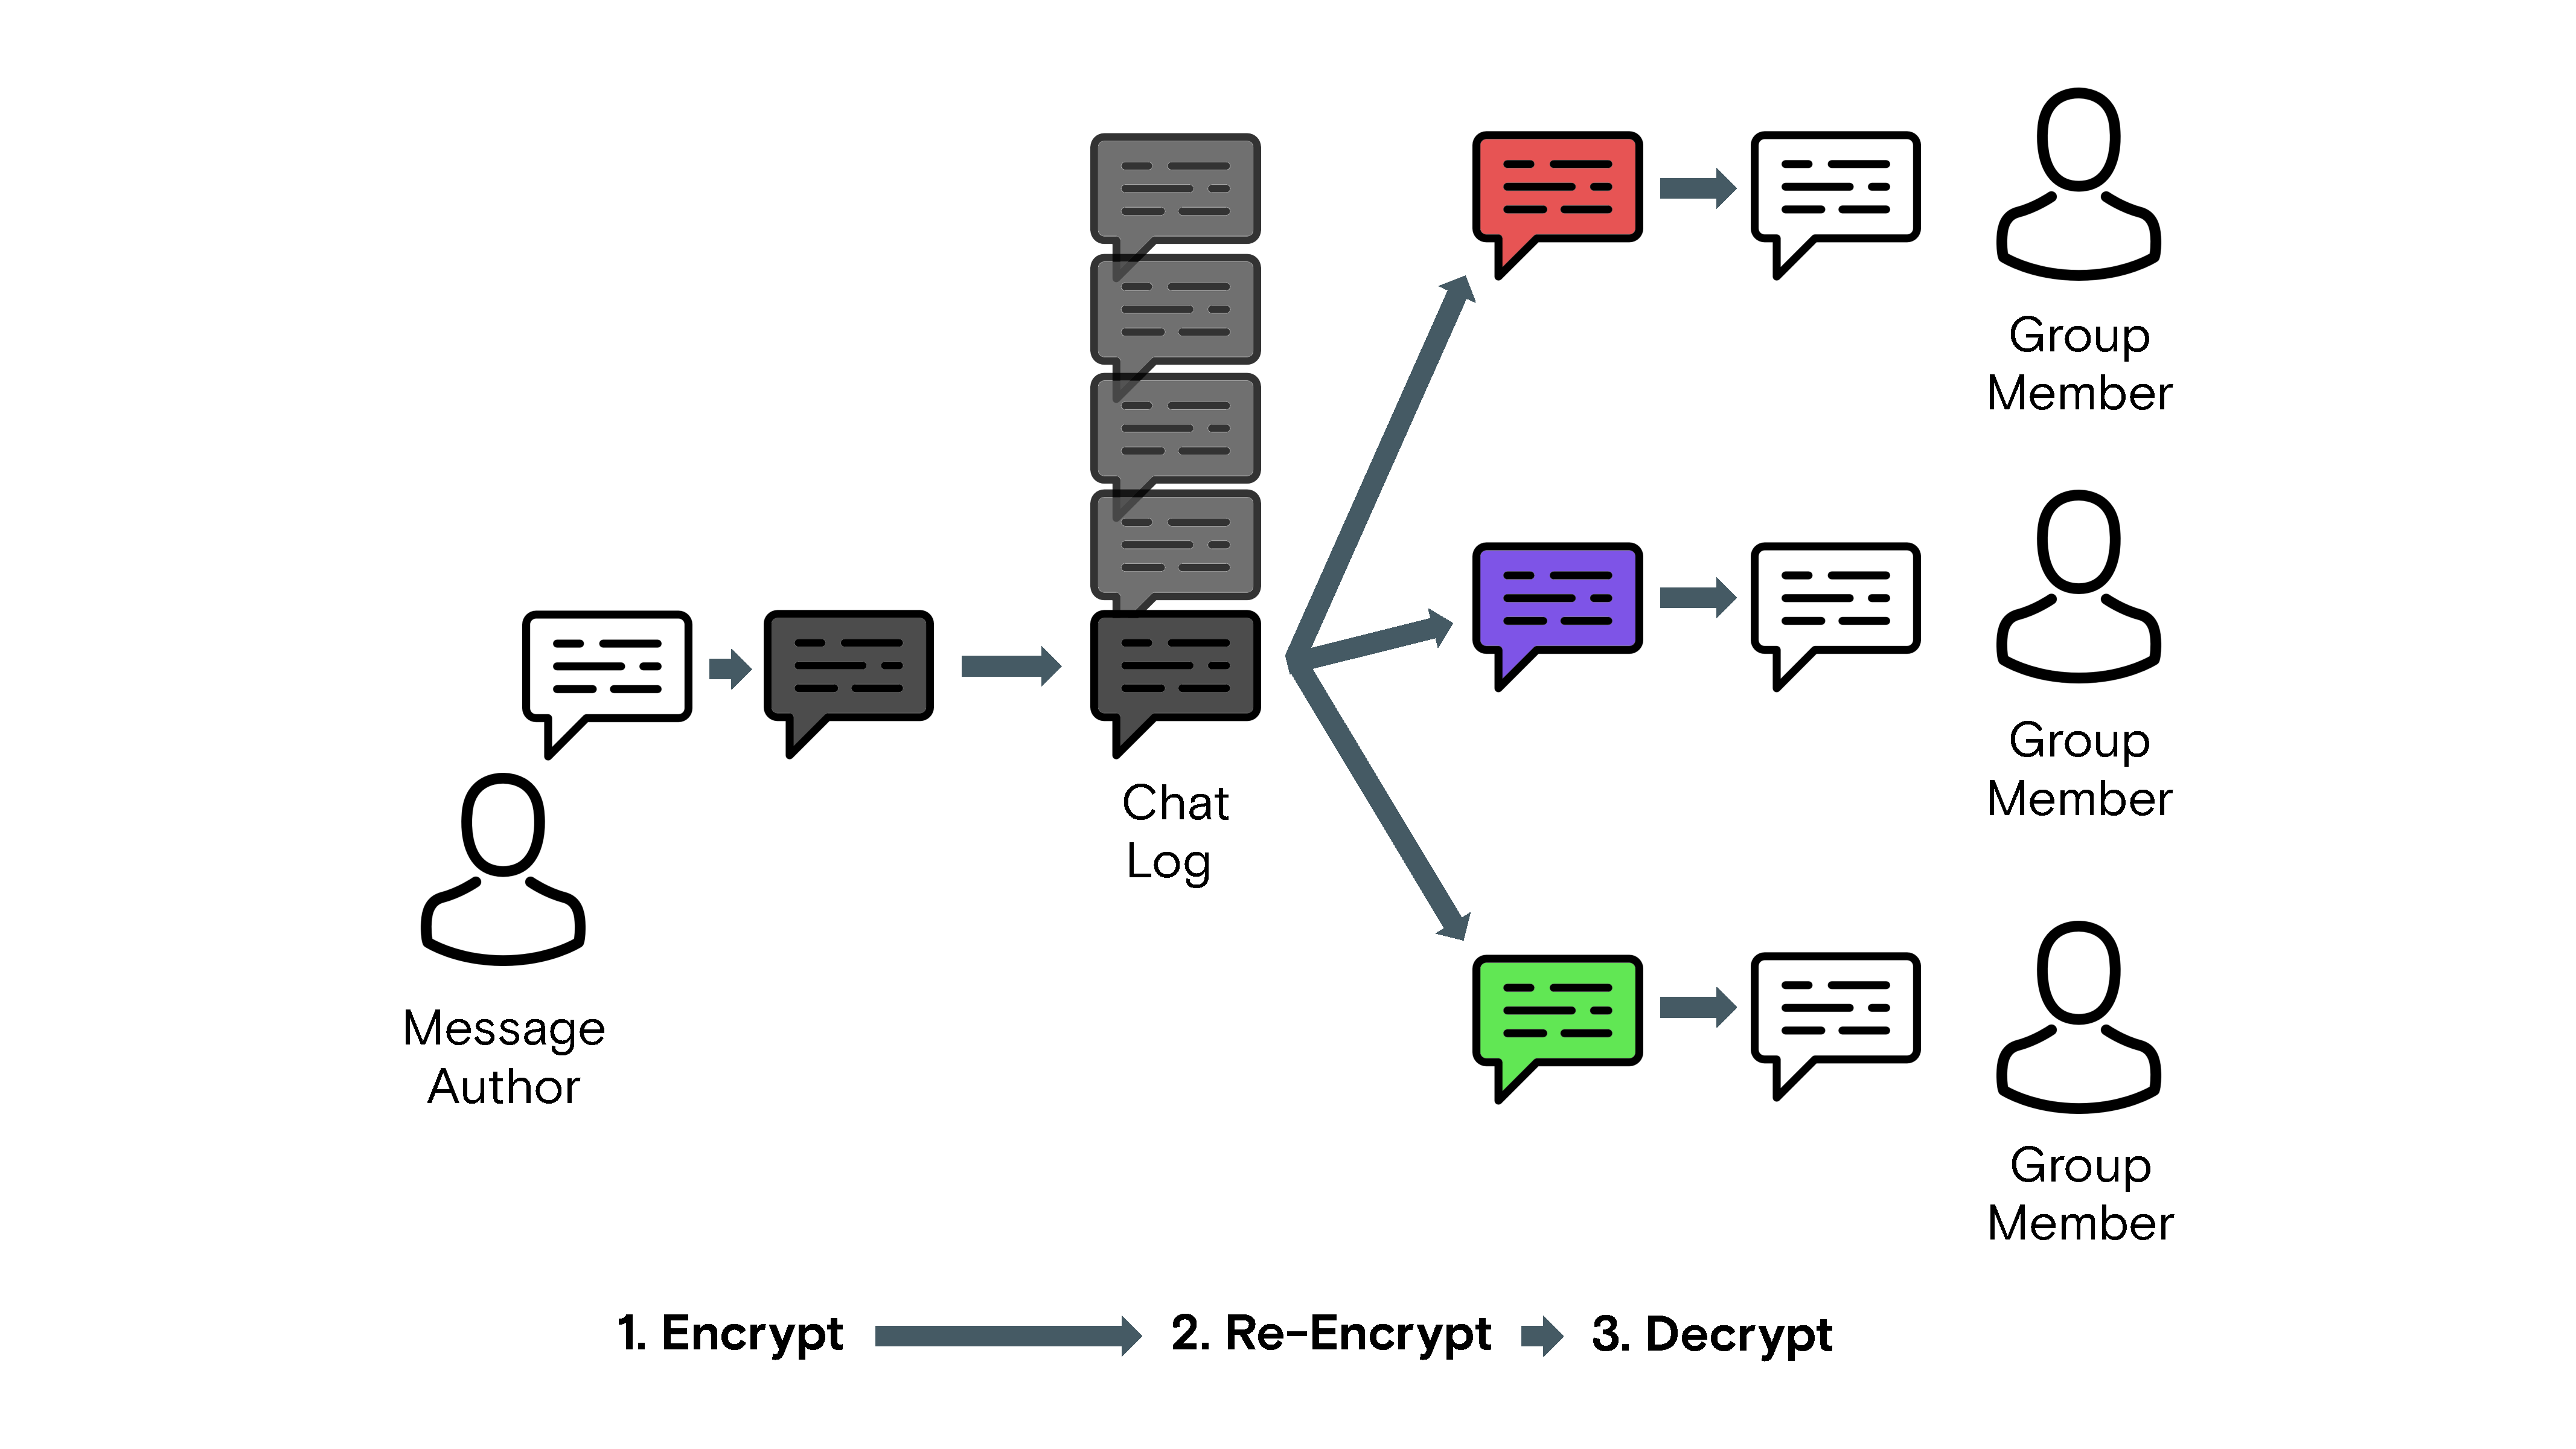
\includegraphics[height=7cm]{pdf/chats-alternative.pdf}
        \end{figure}
    \end{frame}

    \begin{frame}
        \frametitle{Use Cases}
        \framesubtitle{Decentralized access-controlled content}
        \begin{figure}
            \centering
            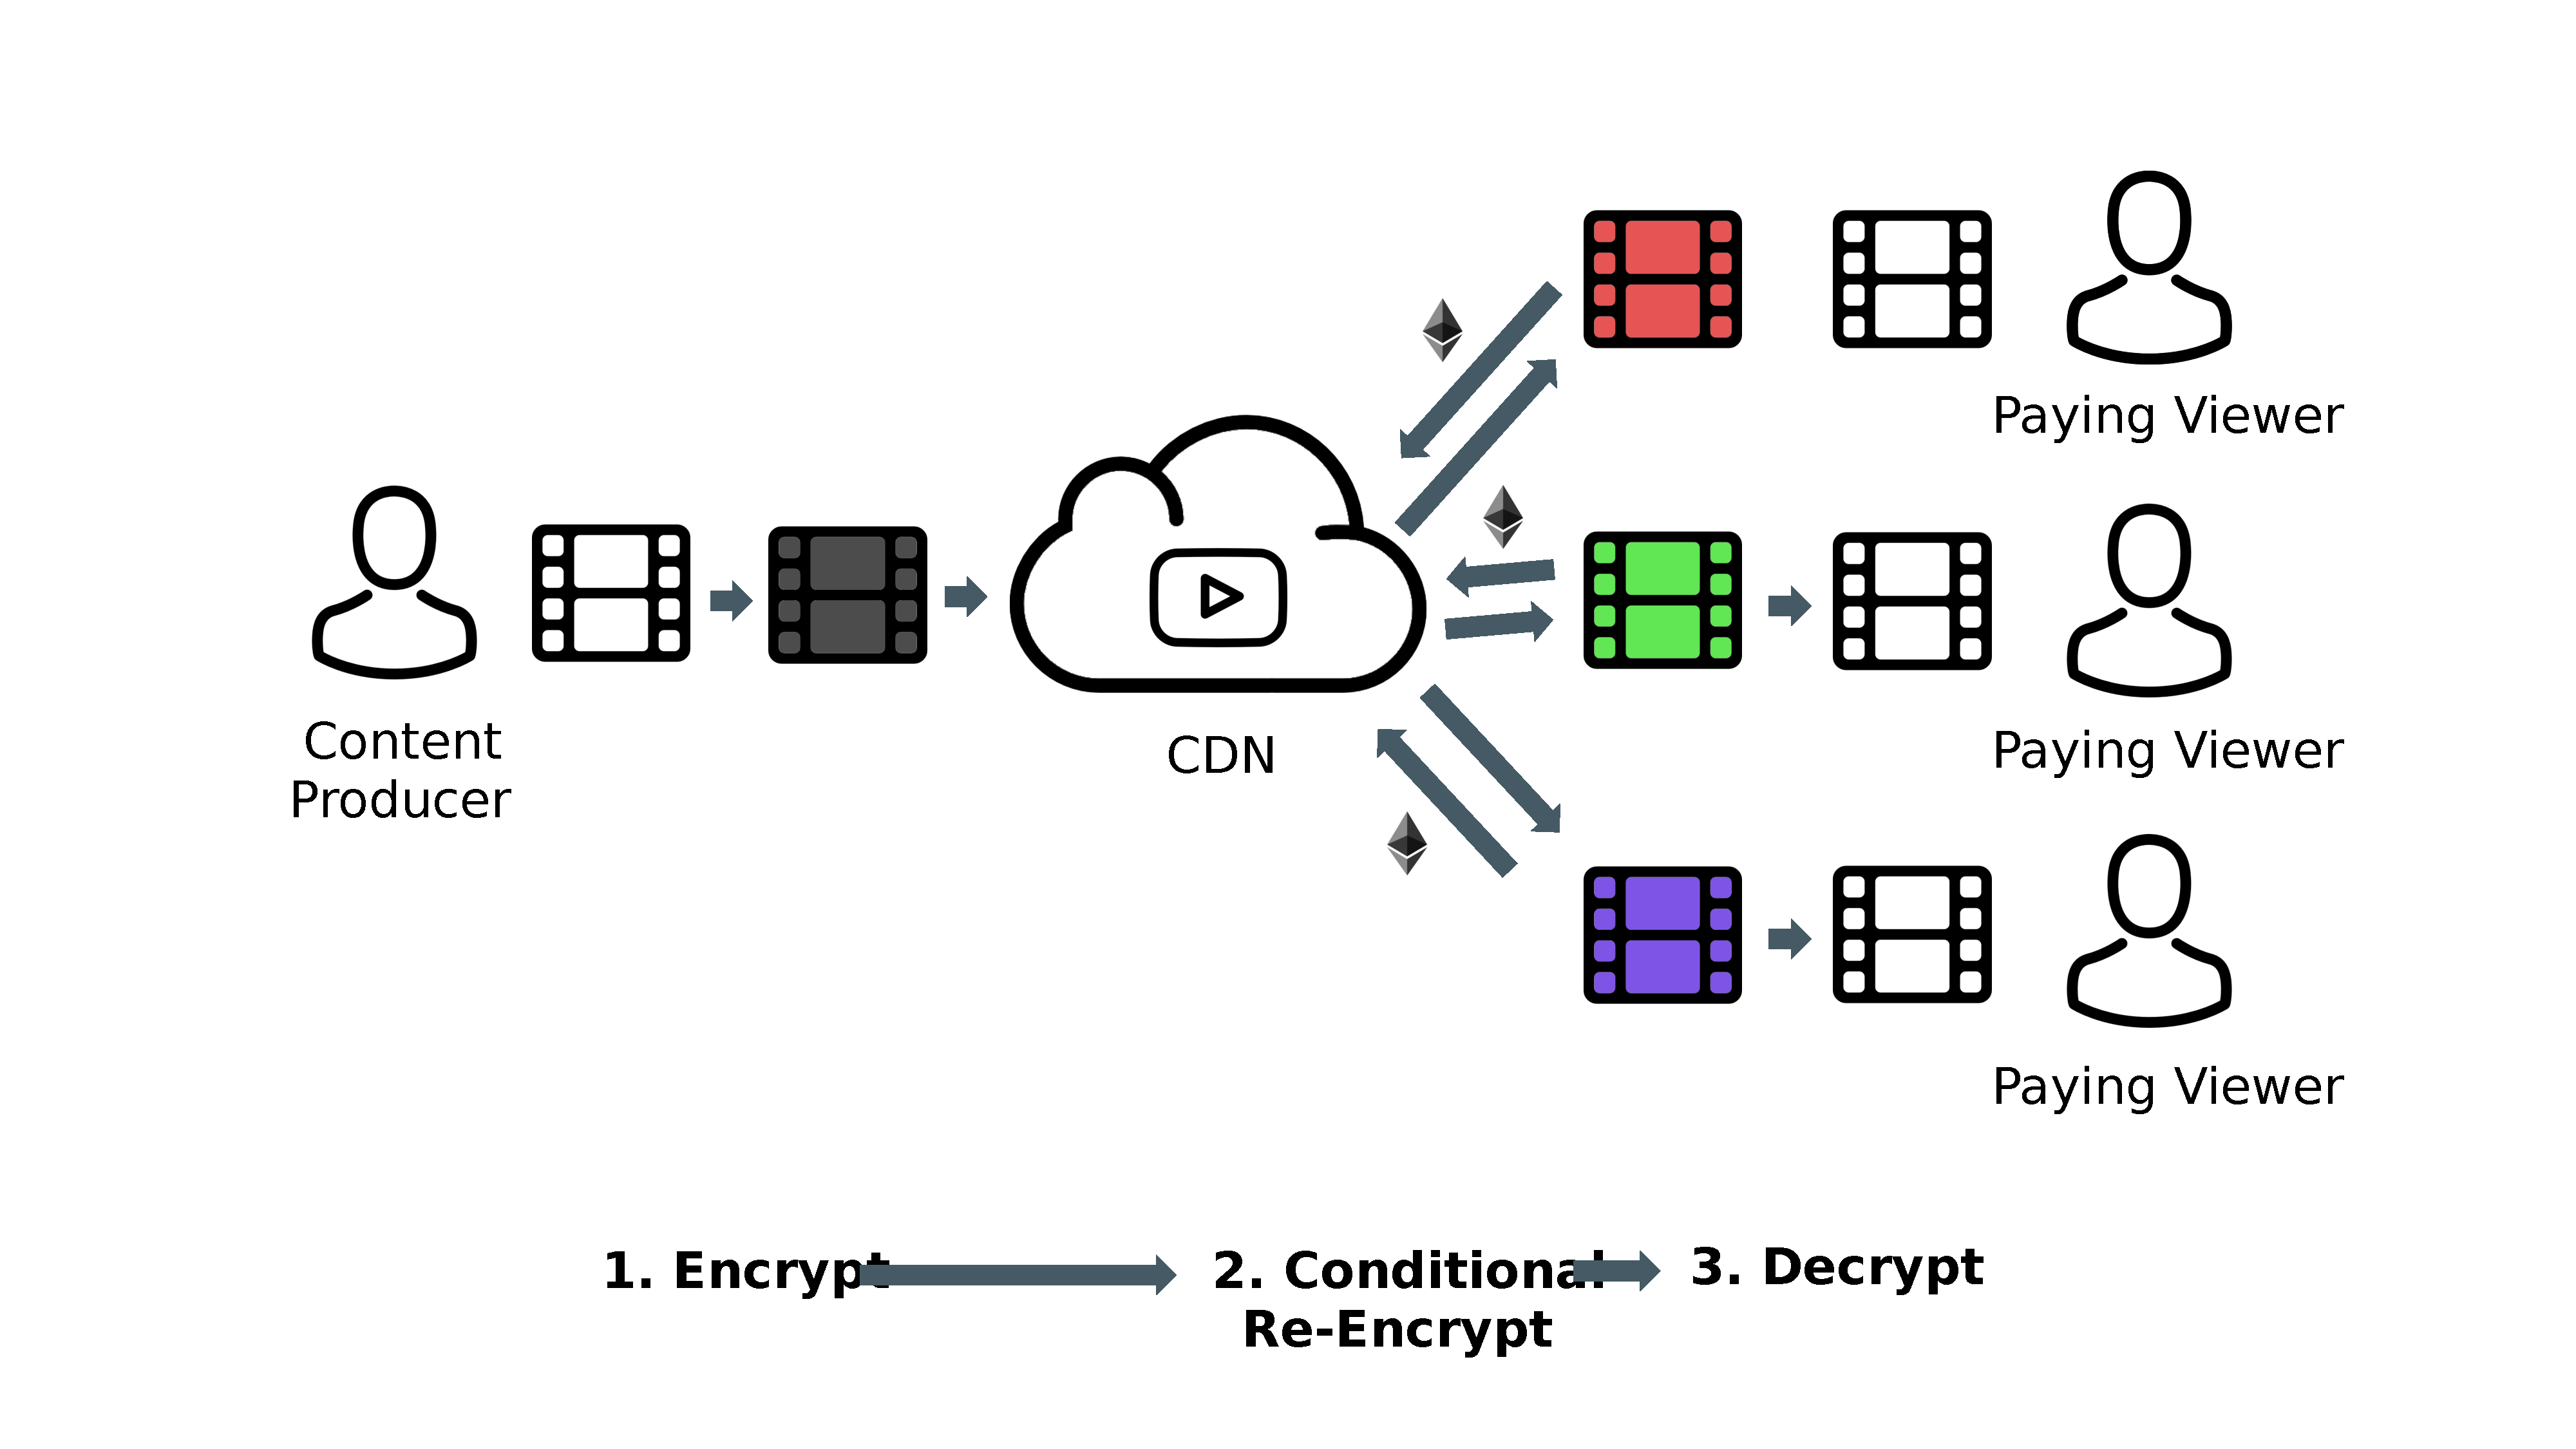
\includegraphics[height=7cm]{pdf/streams-alternative.pdf}
        \end{figure}
    \end{frame}

    \begin{frame}
      \frametitle{Early Users}
      \begin{figure}
           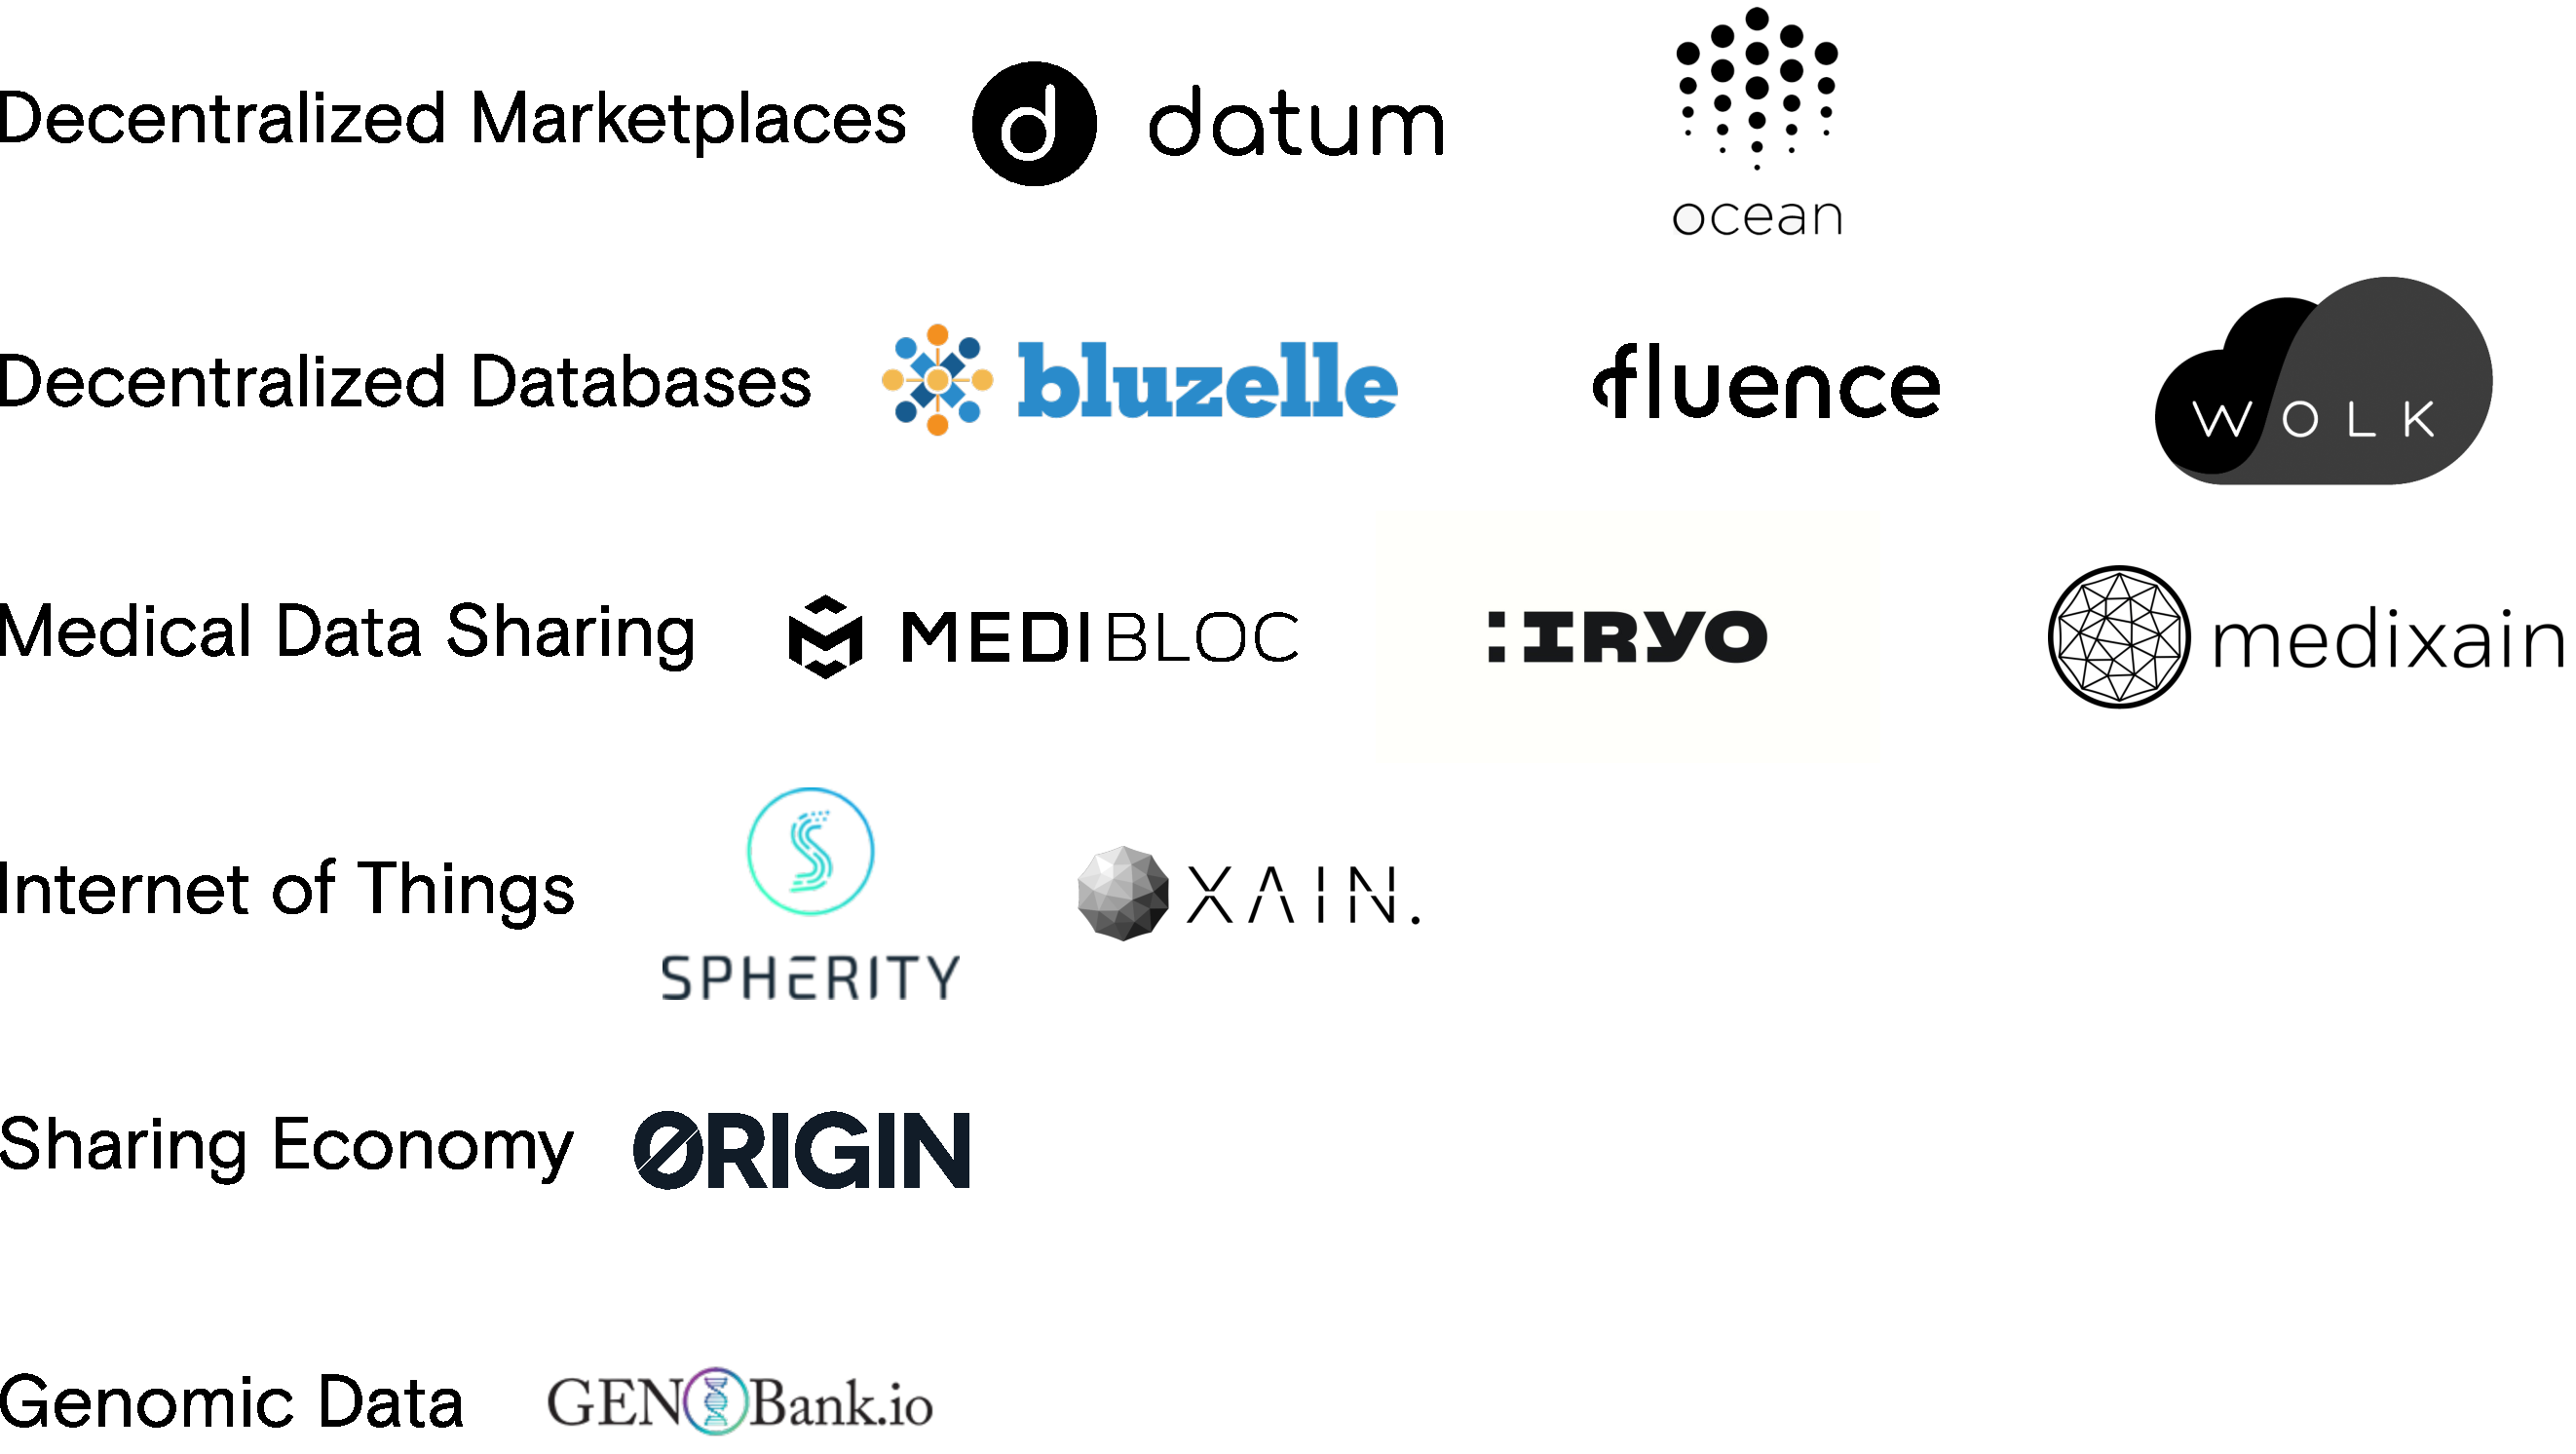
\includegraphics[width=11.5cm]{pdf/projects.pdf}
      \end{figure}
    \end{frame}

    \begin{frame}
        \frametitle{Umbral PRE Demo}
        \begin{figure}
            \centering
            
\includegraphics[height=5.5cm]{pdf/terminal.pdf}
        \end{figure}
        \begin{itemize}
           \item Documentation: \url{https://github.com/nucypher/umbral-doc}
           \item Reference implementation: \url{https://github.com/nucypher/pyUmbral}
        \end{itemize}
    \end{frame}

    \begin{frame}
      \frametitle{Fully Homomorphic Encryption}
       \framesubtitle{nuFHE library}
       \begin{itemize}
           \item GitHub: \url{https://github.com/nucypher/nufhe}
           \item GPU implementation of fully homomorphic encryption
           \item Uses either FFT or integer NTT
           \item Achieved 100x performance over TFHE benchmarks
           \begin{figure}
               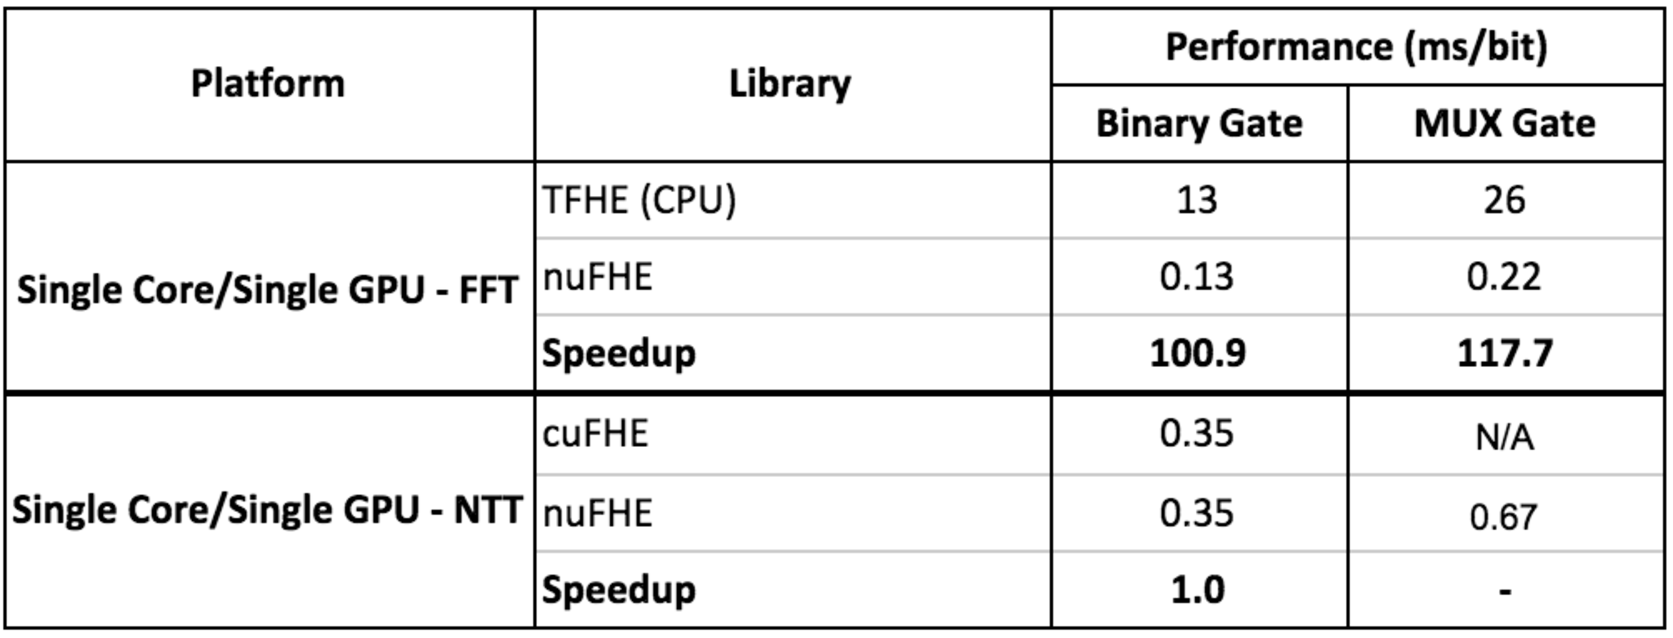
\includegraphics[width=10.5cm]{pdf/nufhe-benchmarks.pdf}
           \end{figure}
       \end{itemize}
     \end{frame}

    \begin{frame}
        \frametitle{More Information}
        \begin{figure}
            \centering
            
\includegraphics[width=3cm]{pdf/nucypher_logo.pdf}
        \end{figure}
        Website: \url{https://www.nucypher.com}

        Whitepaper: \url{https://www.nucypher.com/whitepapers/english.pdf}

        Proxy Re-encryption Network: \url{https://github.com/nucypher/nucypher}

        Umbral Reference Implementation: \url{https://github.com/nucypher/pyUmbral}

        nuFHE: \url{https://github.com/nucypher/nufhe}

        Discord: \url{https://discord.gg/7rmXa3S}

        E-mail: \href{mailto:\emailname @nucypher.com}{\emailname @nucypher.com}

        E-mail: \href{mailto:hello@nucypher.com}{hello@nucypher.com}
    \end{frame}

    \begin{frame}
        \frametitle{Appendix: Umbral - Threshold Proxy Re-encryption}
        \begin{itemize}
        	\item \emph{``Umbral''} is Spanish for \emph{``threshold''}
            \item PRE properties: Unidirectional, single-hop, non-interactive
            \item Follows a KEM/DEM approach:
            	\begin{itemize}
		    \item UmbralKEM provides the threshold re-encryption capability
                    \item Uses ECIES for key encapsulation with ZK proofs of correctness for verifiability on prime order curves (such as secp256k1)
            	    \item DEM can be any authenticated encryption (currently ChaCha20-Poly1305)
        	\end{itemize}
	    \item IND-PRE-CCA security
            \item Key splitting is analogous to Shamir Secret Sharing
	    \item Verification of re-encryption correctness through Non-Interactive ZK Proofs
            \item Reference implementation: \url{https://github.com/nucypher/pyUmbral}
	    \item Documentation: \url{https://github.com/nucypher/umbral-doc}
        \end{itemize}
    \end{frame}

    \begin{frame}
      \frametitle{Appendix: Competing Technology}
       Data Masking and Tokenization
       \begin{itemize}
           \item Less secure for data with underlying patterns
           \item Reduce the value of data by obfuscating it
       \end{itemize}

       Public Key Encryption
       \begin{itemize}
           \item Data must be decrypted before it is shared
           \item Not Scalable
       \end{itemize}

       Multi-Party Computation
       \begin{itemize}
           \item Interactive protocol
           \item Slow Performance
       \end{itemize}

       Fully Homomorphic Encryption
       \begin{itemize}
           \item Slow Peformance
           \begin{itemize}
               \item NuCypher has developed a GPU-accelerated FHE library: nuFHE
           \end{itemize}
       \end{itemize}
     \end{frame}

    \begin{frame}
      \frametitle{Appendix: Fully Homomorphic Encryption}
      \begin{figure}
        \centering
        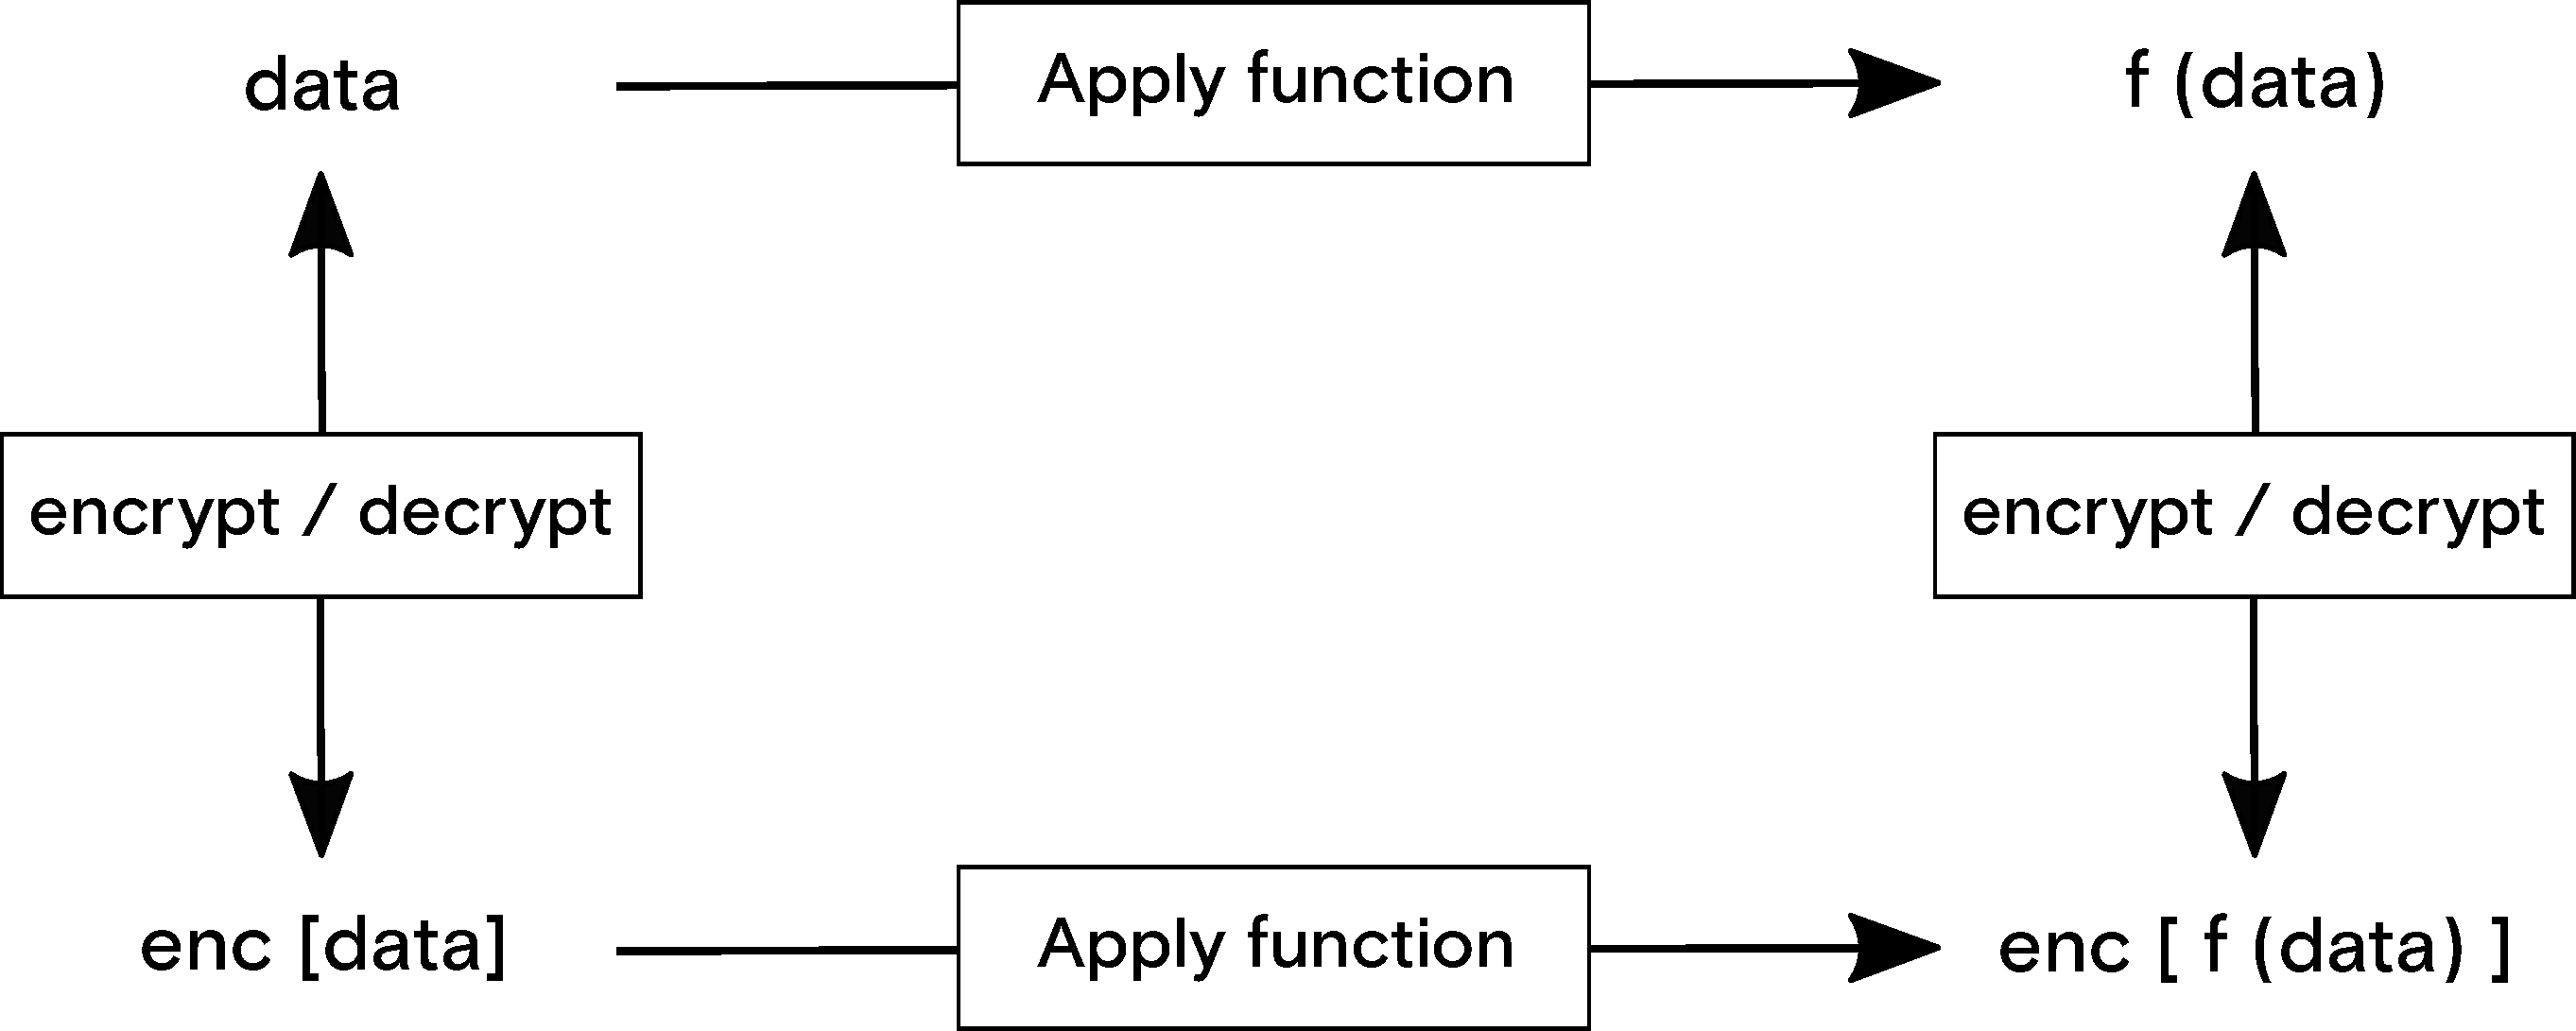
\includegraphics[height=5cm]{pdf/fhe.pdf}
      \end{figure}
    \end{frame}

    \begin{frame}
      \frametitle{Appendix: FHE Proof of Concept}
      \framesubtitle{Sputnik}
      \begin{itemize}
        \item GitHub: \url{https://github.com/nucypher/sputnik}
        \item Assembly language and interpreter for FHE that uses nuFHE
        \item Commits a merkle root of computation to the blockchain for proof of logic flow
        \item Used to execute first homomorphic smart contract at ETHBerlin 2018
      \end{itemize}
      \begin{figure}
        \centering
        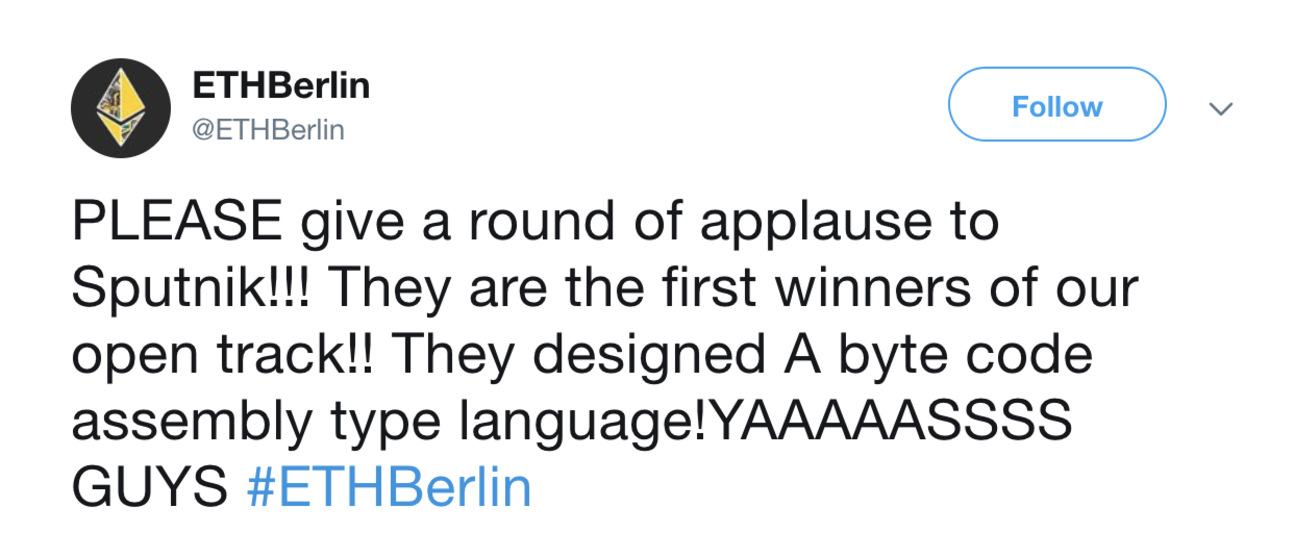
\includegraphics[width=8cm]{pdf/sputnik-tweet.pdf}
      \end{figure}
    \end{frame}

    \begin{frame}
      \frametitle{Appendix: Team}
        \begin{figure}
            \centering
            \includegraphics[width=15cm]{pdf/company.pdf}
        \end{figure}
    \end{frame}

\end{document}


